\documentclass[12pt,letterpaper,spanish]{book}%% Me lo estoy fusilando del demo de winshell.

\usepackage[spanish]{babel} %% Plantilla y separacion de archivos en español.

%\usepackage[latin1]{inputenc} %% Solo windows recuerda cambiar la codificacion de los documentos.
%\usepackage[dvips]{graphicx} %% Para poner figuras cuando se hace el dvi.
\usepackage{ucs}
\usepackage[utf8x]{inputenc} %% Para usar la  directamente los acentos y codificar en utf8

%Este paquete me deja customizar los pies de las figuras y las tablas
\usepackage[margin=2cm,font=footnotesize,labelfont=bf]{caption}

\usepackage{fancyhdr}
%% El paquete geometry es la neta, me deja poner los margenes de manera mas sencilla
\usepackage[left=2cm,right=1.5cm]{geometry}


\usepackage{graphicx} %Imágenes

%%Este hace al momento de hacer el PDF que todas las referencias se conviertan en vinculos
\usepackage[pdftex]{hyperref}

\pagestyle{fancyplain}

%% Redefieniendo las cabezeras y los pies de pagina me lo fusile del demo de winshell
\renewcommand{\chaptermark}[1]
                 {\markboth{#1}{}}
\renewcommand{\sectionmark}[1]
                 {\markright{\thesection\ #1}}
\lhead[\fancyplain{}{\thepage}]
      {\fancyplain{}{\rightmark}}
\rhead[\fancyplain{}{\leftmark}]
      {\fancyplain{}{\thepage}}
\cfoot{}
\sloppy

%% Se supone que esto hace posible poner imagenes en ambos tanto en pdf como en dvi
% \newif\ifpdf
% \ifx\pdfoutput\undefined
%    \pdffalse 
% \else
%    \pdfoutput=1
%    \pdftrue
% \fi
% 
% \ifpdf
%    \usepackage[pdftex]{graphicx}
%    \pdfinfo {
%       /Title (Modelado Grafico de un Cuerpo Neumatico con OpenGL a Base de Ecuaciones Diferenciales)
%       /Subject (Modelado Grafico y Ecuaciones Diferenciales)
%       /Author (Jorge Antonio Garcia Galicia)
%       /Keywords (graficacion, animacion, flexible, ecuacion diferencial, neumatico, opengl)
%    }
% \else
%    \usepackage[dvips]{graphicx}
% \fi

%%paquete que hace que al hacer un pdf, las citas y referencias sean hypervinculos
\usepackage{hyperref}

%% Para quitar un warning que me esta mandando
\setlength{\headheight}{16pt}

\parskip=3mm
%% Empieza el documento

\begin{document}

\author{Jorge Antonio García Galicia}
\title{Modelado Gráfico de un Cuerpo Neumático con OpenGL a Base de Ecuaciones Diferenciales}
\maketitle

\pagenumbering{roman}

\setcounter{page}{1}
\tableofcontents
\listoffigures
\listoftables
\pagenumbering{arabic}

\chapter*{Introducción}
\addcontentsline{toc}{chapter}{Introducción}
\markboth{INTRODUCCIÓN}{INTRODUCCIÓN}

La percepción que tenemos los seres humanos del mundo a través de nuestros sentidos es inmediata. Ademas, dependemos de estos sentidos para realizar la mayoría de las actividades diarias. También hay que señalar que somos criaturas visuales, de nuestros cinco sentidos el que nos proporciona la mayor cantidad de la información que asimilamos sin lugar a dudas son nuestros ojos \cite{Hagen:vista}.

Desde hace mas de tres décadas las computadoras se han vuelto mas poderosas y hemos tenido la oportunidad de procesar con ellas una mayor cantidad de datos de manera rápida. Una de las áreas que se ha encontrado mas beneficiada es la imagenología biomédica. Si bien es cierto que los rayos X eran desde hace mucho una herramienta probada para el diagnostico médico (y diversas aplicaciones industriales), una imagen digital que pudiera almacenarse, procesarse y luego desplegarse en una computadora ha sido un parteaguas para este campo. Al mismo tiempo, muchas áreas de las ciencias de la computación (CC) han cobrado interés durante el mismo periodo. Particularmente, el procesamiento de imágenes digitales, las gráficas por computadora y la visualización científica, son ahora una opción viable para usarse rutinariamente.

El procesamiento de imágenes estudia como procesar imágenes digitales por medios computacionales \cite{Gonzalez:ImagenesDigitales}. Algunas veces este proceso implica transformar una imagen en otra imagen en donde se ha resaltado, o inhibido, cierta característica. Otras veces implica obtener otro tipo de información de una imagen, por ejemplo un histograma. Finalmente, algunas veces implica poder distinguir o interpretar datos de objetos a partir de las imágenes.

Las gráficas por computadora (GC) son la rama de las CC que estudia las técnicas para producir imágenes digitales a partir de descripciones matemáticas. Estas imágenes son visualizadas en dispositivos de despliegue en 2D, por ejemplo un monitor, por lo que generalmente es necesario hacer una proyección de los objetos (en tres dimensiones) a un plano.

La visualización científica se encarga de construir información visual de conjuntos de datos científicos. Estos datos pueden tener orígenes muy diversos; inclusive pueden simular fenómenos de la naturaleza que no pueden ser percibidos por nuestra vista. Por ejemplo, ver en la pantalla el espacio de solución de una ecuación diferencial que modele la vibración de la cuerda de una guitarra es un problema de visualización científica que se podría equiparar con la idea de ``visualizar la música''.

En éste trabajo se abarca un poco de estas tres áreas. Asumimos que tenemos un conjunto de datos distribuidos en un arreglo cúbico que representan un muestreo de un campo escalar tridimensional. Estos datos forman lo que típicamente se conoce como una imagen digital en 3D o volumen. Debido a la naturaleza de los datos nos interesa poder visualizarlos sin perder su información espacial.

%La manera como haremos esto es realizando una segmentación que nos permita extraer una superficie de la imagen y luego pretendemos visualizar esa superficie. Lo primero es encontrar una malla que se aproxime a la superficie. Para esto se hace uso de un algoritmo de extracción de superficies propuesto por Herman y Artzy en \cite{ArtzyLargo}. Este algoritmo tiene la desventaja de obtener una aproximación a las superficie formada por caras de cuadrados orientadas ortogonalmente. Por esta razón los resultados se ven como si fueran bloques de LEGO\textcopyright.
Una forma de lograr éste objetivo es encontrar una superficie que defina la frontera de un objeto y luego visualizar la superficie como si ésta fuera un envolvente. Como en un principio se tiene la imagen en 3D es necesario utilizar algún criterio que defina la superficie (proceso típicamente conocido como segmentación). Dado la naturaleza del volumen debemos encontrar una manera de generar un conjunto de polígonos para aproximar la superficie de manera digital.

En este trabajo estudiaremos dos métodos para aproximar esas superficies: el algoritmo de \emph{Marching Cubes} \cite{MarchingCubes}, que es el mas usado actualmente, y el Algoritmo de Artzy \cite{artzyCorto}. El Algoritmo de Artzy tiene varias ventajas sobre el primero, la mas importante es que garantiza que la superficie aproximada es topológicamente correcta, es decir que no contiene agujeros. Sin embargo, la desventaja mas importante de Artzy es que las mallas obtenidas parecen cuboides, como si fueran hechas por bloques del juego de LEGO.%$^\copyright$.

Sin importar el método de obtención de la malla, se visualiza por medio de técnicas de graficación por computadora. Esto incluye utilizar \emph{iluminación}, que en conjunto con otras técnicas, tiene la función de dar la apariencia de 3D a la proyección en 2D. Para poder utilizar la iluminación es necesario que proporcionemos un conjunto de vectores normales a la superficie en cada vértice de la malla. Como es mostrado en la técnica conocida como \emph{bump mapping} \cite{bussCG}, estos vectores pueden afectar significativamente la apariencia final de la imagen.

En este trabajo proponemos una forma de obtener un conjunto de vectores normales en los vértices de la malla obtenida por el Algoritmo de Artzy, tales que al usarse en conjunto con la iluminación, el resultado final sea una apariencia mas suave del objeto. Por lo tanto se obtendría una malla que conserva las ventajas del Algoritmo de Artzy pero que sea visualmente equiparable con la malla producida por \emph{Marching Cubes}. Para esto, pensamos encontrar un envolvente suave de la malla por medio de funciones base de transición suave de uno a cero; conocidas como Kaiser Bessel generalizadas.

La organización del trabajo es la siguiente. En el primer capítulo, se hace la fundamentación matemática necesaria de lo que entendemos como volumen y se explican que condiciones esperamos que cumplan los volúmenes de los que hablamos en el resto del trabajo. También se analizan los dos algoritmos de rastreo de superficies sobre volúmenes antes expuestos poniendo énfasis en las propiedades presentes en el Algoritmo de Artzy. También se revisa el modelo de iluminación de Phong y se habla de los modelos de sombreado de Phong y de Gouraud. Por último se revisan dos técnicas de GC que usan mapas para dar efectos: el mapeo de texturas y el mapeo de relieves (\emph{bump mapping}).

En el segundo capítulo se introducen las superficies implícitas y algunas funciones base que comúnmente se usan para crear dichas superficies. Luego se introducen las funciones Kaisser Bessel generalizadas que servirán de funciones base en el resto del trabajo. También se exponen las contribuciones del trabajo. La primera es que se sigue el método de optimización para funciones base propuesto en \cite{EdgarOptimization} y se llegan a parámetros óptimos para tres casos. La segunda aportacion es que se obtiene un algorimo para crear la superficie implícita que envuelva la malla producida por el Algoritmo de Artzy y como se le asignan normales a los vértices de esa malla. Esta última es la principal aportación del trabajo.

El tercer capítulo esta dedicado a los experimentos realizados para probar la metodología expuesta. En primer lugar se muestran resultados puramente visuales sobre algunos conjuntos de datos provenientes de imagenología biomédica. Posteriormente, se explica la manera como se construyen dos \emph{phantoms} (un cubo y una esfera) a diferentes resoluciones y se evalúan las diferencias entre las normales analíticas de los \emph{phantoms} y las obtenidas por nuestro método.

Por último, en el capítulo final se presentan las conclusiones del trabajo y conjuntamente se proponen lineas de investigación futuras.

\subsubsection*{Objetivos del trabajo}

El principal objetivo de este trabajo es encontrar por medio de la modificación de normales una forma de hacer la superficie obtenida por el Algoritmo de Artzy visualmente mas agradable. Haciendo enfasis en que no hacemos ninguna suposición sobre como fue la discretización del volumen.


\chapter{Visualización de imágenes 3D}
\label{chap:visualizaImagenes}
En éste trabajo estamos interesados en visualizar campos escalares discretizados. Un campo escalar es un mapeo $f:\mathbb{R}^3 \rightarrow \mathbb{R}$ donde $f$ típicamente representa el valor de una cantidad física en el espacio. En la actualidad muchos dispositivos, por ejemplo los tomógrafos, son capaces de producir muestreos de estos campos. Dada la naturaleza electrónica de los dispositivos con los que medimos el campo escalar, en realidad se tiene una aproximación de $f$ que se obtiene, en general, muestreando de manera uniforme el espacio tridimensional. 

%Sean $I, J, K \in \mathbb{Z}^+$. Para todo $\langle i, j, k \rangle \in \left[ 1, I \right] \times \left[ 1, J \right] \times \left[ 1, K \right]$ y para todo $d \in \mathbb{R}^+$, definimos un vóxel como:
Para representar un punto en $\mathbb{R}^n$, alternativamente $\mathbb{Z}^n$, usaremos la representación $\textbf{p} \in \mathbb{R}^n$, alternativamente $\textbf{k} \in \mathbb{Z}^n$, y su $n$-tupla $\textbf{p} = \{ p_1, p_2,\ldots, p_n \}$ donde $p_i \in \mathbb{R}$, alternativamente $\textbf{k} = \{ k_1, k_2,\ldots, k_n \}$ donde $k_i \in \mathbb{Z}$. Debido a que usamos recursos finitos para llevar a cabo la discretización de $f$ solo usaremos un subconjunto $\Gamma \subset \mathbb{Z}^3$ definido de la siguiente manera:

\begin{equation}
\Gamma = \left\lbrace \textbf{k} | A_i \leq k_i \leq B_i \text{ para } 1 \leq i \leq 3 \text{ con } A_i < B_i \text{ y } A_i, B_i \in \mathbb{Z} \right\rbrace 
 \label{ec:escena}.
\end{equation}

Dado un punto $\textbf{k} \in \Gamma$ y un numero real positivo $\Delta$, definimos un vóxel cúbico como 
\begin{equation}
   \text{Vox} (\textbf{k}) = \left\lbrace \textbf{x} \in \mathbb{R}^3 | \Delta \left(  k_i - \dfrac{1}{2} \right) \leq x_i < \Delta \left(  k_i + \dfrac{1}{2} \right)  , \text{ para } 1 \leq i \leq 3 \right\rbrace 
  \label{ec:voxel},
\end{equation}al número $\Delta$ comúnmente se le conoce como distancia de muestreo\cite{edgarReconstruction}. El termino vóxel proviene del ingles \emph{volume element} y por lo tanto pueden existir vóxeles no cúbicos. Al mismo tiempo un punto $\textbf{k} \in \mathbb{Z}^2$ tiene asociado un píxel, proveniente del ingles \emph{picture element}. Debido a que en éste trabajo no utilizamos teselaciones no cúbicas, usaremos el término vóxel para referirnos a los vóxeles de \eqref{ec:voxel}.

Al subconjunto $\Gamma$ de $\mathbb{R}^3$ para el cual esta definido $v$ se le llama \emph{escena}. De manera convencional a cada uno de los límites de las dimensiones del dominio de $v$ se le da un nombre. Típicamente al intervalo valido de $k_1$ se le conoce como el \emph{ancho} de la imagen, al intervalo de $k_2$ como la \emph{altura} de la imagen y al de $k_3$ como la \emph{profundidad} de la imagen.

Los vóxeles también pueden verse como la vecindad de Voronoi de un conjunto de puntos dispuestos como un arreglo rectangular que llena la escena\cite{Gabor:DigitalSpaces}, a este arreglo de puntos lo llamamos rejilla cúbica simple (\emph{sc}). Aunque de momento solo se hace uso de rejillas \emph{sc} estas no son las únicas formas de muestrear de manera uniforme el espacio, también existen otras rejillas como la \emph{face-centered cubic grid} (\emph{fcc}) o la \emph{body-centered cubic grid} (\emph{bcc}) que cubren el espacio de vóxeles con forma de rombo dodecaedros y de octaedros truncados respectivamente \cite{Gabor:DigitalSpaces}.

%Se hace la aclaración de que el término vóxel viene de \emph{volume element}, que es una generalización de su análogo de dos dimensiones \emph{píxel} de \emph{picture element}. A la teselación del espacio $\mathbb{R}^3$ en vóxeles como están definidos en la ecuación \eqref{ec:voxel} se le conoce como \emph{rejilla cúbica simple} (sc). A la distancia $d$ la llamamos \emph{distancia de muestreo}.

Dado un campo escalar $f$ y un intervalo de muestreo $\Delta$, definimos una digitalización como
\begin{equation}
  p_{\Delta}( \textbf{k} ) = \dfrac{1}{\Delta^3} \int \limits_{\text{Vox} ( \textbf{k} )} f(\textbf{x}) d\textbf{x}.
  \label{ec:digitalizacion}
\end{equation}

La digitalización definida en \eqref{ec:digitalizacion} da origen a una \emph{imagen digital} en 3D (o \emph{volumen}) que se define de la siguiente manera:
\begin{equation}
  v(\textbf{k}) =
  \begin{cases} 
      p_{\Delta}(\textbf{k}), & \text{ si } \textbf{k} \in \Gamma, \\
      0, & \text{ en otro caso.} \\                                
    \end{cases}
  \label{ec:imagen3D}
\end{equation}

Se espera que la imagen digital $v$ sea una buena aproximación del campo escalar $f$. Para que esto último sea posible deben pasar dos cosas. Primero que la distancia $|B_i - A_i|$ sean lo suficientemente grande como para abarcar todo el rango de interés del campo escalar $f$ y segundo, que la distancia $\Delta$ sea lo suficientemente pequeña para que los detalles importantes de la imagen no se pierdan debido a la digitalización expresada en \eqref{ec:digitalizacion} \cite{edgarReconstruction}. La principal limitante para lograr estas condiciones es que dependemos de la capacidad del dispositivo y de los algoritmos con los que se hace la digitalización. En este trabajo, sin embargo, se asumirá que no se tiene control del dispositivo del que se obtienen las imágenes, pero que se han obtenido ``buenas'' aproximaciones.

Al valor escalar $p_{\Delta}(\textbf{k})$ definido en \eqref{ec:digitalizacion} se le asocia una cantidad física que generalmente tiene que ver con la detección de la interacción de la materia que haya en el vóxel $\textbf{k}$ con cierta radiación. Aunque los tomógrafos proporcionan un valor $v(\textbf{k}) = \lambda \in \mathbb{R}$, algunas veces escalamos el rango de valores $r_i \leq \lambda \leq r_f$ a un cierto intervalo $[0, 2^i - 1]$ para algún entero positivo $i$.

En áreas como la medicina y la biología es común visualizar los volúmenes $v$ por planos o cortes generados al dejar fijo algún valor $k_i$ para alguna escena $\Gamma$. En medicina, si se trata de un volumen $v$ que aproxima un ser humano visto de pie, es común llamar a estos cortes como \emph{coronal} si divide al cuerpo humano en dos secciones adelante y atrás, \emph{sagital} si divide al cuerpo humano en secciones izquierda y derecha y \emph{axial} si lo divide en secciones arriba y abajo, ver Figura \ref{fig:cortesHB}. Sin embargo, este tipo de visualización tiene la enorme desventaja de perder la estructura tridimensional de la imagen, ver la Figura \ref{fig:imagenDigital}.

\begin{figure}[htp]
 \centering
  \includegraphics[scale=0.4]{img/cap01/HumanAnatomyPlanes}
  \caption[Cuerpo humano dividido en planos sagital, axial y coronal (La imagen fue tomada de \cite{wikiImagen})]{Cuerpo humano dividido en planos sagital, axial y coronal (La imagen fue tomada de \cite{wikiImagen}).}
  \label{fig:cortesHB}
\end{figure}

\begin{figure}[htp]
 \begin{center}
    \subfigure{\includegraphics[scale=0.45]{img/cap01/01}}
    \subfigure{\includegraphics[scale=0.45]{img/cap01/02}} 
    \subfigure{\includegraphics[scale=0.45]{img/cap01/03}} \\
    \subfigure{\includegraphics[scale=0.45]{img/cap01/04}}
    \subfigure{\includegraphics[scale=0.45]{img/cap01/05}} 
    \subfigure{\includegraphics[scale=0.45]{img/cap01/06}}
  \end{center}
  \caption[Un volumen o imagen 3D visualizada por planos sagitales de una cabeza obtenida por medio de MRI (obtenida de \cite{visualHumanSite})]{Un volumen o imagen 3D visualizada por planos sagitales de una cabeza obtenida por medio de MRI (obtenida de \cite{visualHumanSite}).}
  \label{fig:imagenDigital}
\end{figure}

Por esta razón se han desarrollado formas de hacer una visualización completa de las imágenes que preserve la estructura 3D. Hay dos métodos generales de atacar este problema. La primera forma es conocida como visualización directa o \emph{volume rendering}. Este método fue originalmente propuesto por Drebin, Loren y Hanrahan en \cite{VolumeRendering} y hace uso de una técnica de GC conocida como \emph{alpha blending}. El método consiste en asociar a los vóxeles en la imagen $v$ una cierta función de transferencia y con ella calcular para cada vóxel $\textbf{k}$ un valor alfa (o de transparencia), de esta manera vóxeles con valores $p_{\Delta}( \textbf{k} )$ diferentes adquieren diferentes grados de opacidad. Esto permite ver todo el volumen directamente como una colección de objetos translúcidos. Un ejemplo se muestra en la Figura \ref{fig:volRender}.

\begin{figure}[htp]
 \centering
  \includegraphics[scale=0.5]{img/cap01/volRender}
  \caption[El mismo conjunto de datos de la Figura \ref{fig:imagenDigital} visualizado por Volume Rendering]{El mismo conjunto de datos de la Figura \ref{fig:imagenDigital} visualizado por Volume Rendering. En esta imagen se usa el método de suma de intensidades como función de transferencia.}
  \label{fig:volRender}
\end{figure}

El otro método de visualización se llama \emph{visualización indirecta} o por superficies. Dado un campo escalar $f(\textbf{x})$, donde $f$ es una función escalar de $\mathbb{R}^3$, se define una superficie como sigue
\begin{equation}
S_{\tau} = \left\lbrace \textbf{x} \: | \: f(\textbf{x}) = \tau \right\rbrace 
 \label{ec:isosupeficie}.
\end{equation}
La superficie $S_{\tau}$ es llamada \emph{isosuperficie} o \emph{frontera} definida por $\tau$; el valor constante $\tau$ es llamado \emph{isovalor} o \emph{umbral}. Debido a que tenemos la aproximación $v$ de $f$, las técnicas por isosupeficie consisten en seleccionar un isovalor del conjunto de $p_{\Delta}(\textbf{k})$ (el rango de la imagen)  y rastrear la isosuperficie definida por ese valor. Esto resulta en una especie de envolvente o cascara discreta que forma una malla poligonal. Para poder definir la malla es necesario tener los vértices de cada polígono y la conectividad (saber que par de vértices forman cada arista). Esta malla se puede visualizar por métodos tradicionales de GC. En la Figura \ref{fig:visIsoSurface} se muestra el mismo volumen de las Figuras \ref{fig:imagenDigital} y \ref{fig:volRender} visualizado por cuatro isosuperficies correspondientes a diferentes isovalores en el rango $[0,255]$ y con el método de \emph{Marching Cubes}, explicado mas adelante.

  \begin{figure}[htp]
  \begin{center}
    \subfigure[$\tau = 61$]{\label{fig:mc61}\includegraphics[scale=0.4]{img/cap01/mc61}}
    \subfigure[$\tau = 69$]{\label{fig:mc69}\includegraphics[scale=0.4]{img/cap01/mc69}} \\
    \subfigure[$\tau = 83$]{\label{fig:mc83}\includegraphics[scale=0.4]{img/cap01/mc83}}
    \subfigure[$\tau = 123$]{\label{fig:mc123}\includegraphics[scale=0.4]{img/cap01/mc123}}
  \end{center}
  \caption[Visualización por superficies de la imagen 3D de la Figura \ref{fig:imagenDigital} con cuatro isovalores distintos]{Visualización por superficies de la imagen 3D de la Figura \ref{fig:imagenDigital} con cuatro isovalores dentro del rango $[0,255]$ producida con el método de \emph{Marching Cubes}.}
  \label{fig:visIsoSurface}
  \end{figure}

Hay varias razones por las que la visualización por superficies es más usada. Por ejemplo la rapidez del cómputo y el hecho de que tanto el hardware como el software que usamos esta optimizado para visualizar estas superficies. Sin embargo, la mas importante es que los humanos estamos acostumbrados a ver las cosas de esa manera, generalmente solo percibimos la capa exterior de la mayoría de los objetos.
%El Algoritmo de Artzy tiene bastantes propiedades deseables ausentes en MC. Sin embargo, dado que éste último es el estándar contra el cual compararemos los resultados del trabajo es conveniente tener claro como funcionan ambos algoritmos.
\section{Generación de mallas}
\label{sec:generarMallas}
Hay varios algoritmos que pueden rastrear la frontera y construir la malla que la aproxima. El algoritmo de \emph{Marching Triangles}, propuesto por Hilton,  Stoddart, Illingworthy y Windeatt en \cite{marchingTriangles}, produce una malla a partir de una nube de puntos. En este algoritmo se empieza con un triangulo y se empiezan a añadir vértices que forman triángulos con las aristas que ya pertenecen a la malla, cuidando de cumplir que la triangulación que forma la malla sea siempre una triangulación de Delaunay. Este método tiene la enorme ventaja de producir mallas estables y de buena calidad. La desventaja de este algoritmo es que la malla resultante no suele adaptarse bien a las secciones de la superficie donde hay muchos detalles finos. En \cite{regionGrowingExtraction} se propone una mejora, capaz de producir mallas adaptables y además es capaz de encontrar los diferentes componentes conexos del volumen.

Otro algoritmo que fue propuesto por Keppel \cite{contoursKeppel} reconstruye la superficie a través de secciones transversales del volumen. En un primer paso en cada una de las secciones transversales extraen un contorno por medio de algún algoritmo de detección de bordes. En un segundo paso los contornos de secciones adyacentes se empiezan a unir formando polígonos. El paso crucial de este algoritmo es conectar de manera correcta los diferentes contornos. Sin embargo, debido a que los contornos que deseamos reconstruir en medicina son muy complejos no se logra hacer la conexión de manera aceptable. Por esto último se han escrito algunas mejoras (ver por ejemplo \cite{improvementCoutours}), pero debido a que la mayoría se basan en heurísticas estos métodos son poco usados en la actualidad \cite{focOnSciVis}. 

En éste trabajo estamos interesados en dos métodos: el método de \emph{Marching Cubes} (MC)\cite{MarchingCubes} que es el estándar mas usado actualmente y el Algoritmo de Artzy\cite{artzyCorto}.

\subsection{Adyacencias y caminos}

Antes de explicar como funcionan estos algoritmos necesitamos definir los conceptos de adyacencia y camino entre vóxeles

El concepto de \emph{adyacencia} entre dos vóxeles es una relación binaria simétrica sobre $\mathbb{Z}^3$. Se dice que dos vóxeles son vecinos cuando son adyacentes. Existen varias adyacencias, aquí solo vamos a utilizar dos de las más comunes.

Se dice que dos vóxeles $\textbf{c}$ y $\textbf{d}$ en la rejilla \emph{sc} son \emph{adyacentes cara a cara} o $\omega$-adyacentes, si difieren en sólo una de sus coordenadas, ver Figura \ref{fig:omegaAdyacencia}. Es decir:
\begin{equation}
(\textbf{c}, \textbf{d}) \in \omega \leftrightarrow |\textbf{c} - \textbf{d} | = 1 
\label{ec:adja6},
\end{equation} en donde $|\textbf{p}|$ denota la norma euclideana del vector $\textbf{p}$. Un vóxel en la rejilla puede ser adyacente bajo $\omega$ con otros seis vóxeles de la rejilla, es por eso que a esta adyacencia se le conoce también como la $6$-vecindad del vóxel, ver la Figura \ref{fig:vec6vecindad}.

%Otra posible adyacencia es la llamada \emph{adyacencia vértice a vértice} ó $\alpha$-adyacencia. Aquí se dice que dos vóxeles son adyacentes si comparten una cara, si comparten una arista, o bien si comparten un vértice. Ver Figura \ref{fig:alphaAdyacencia}. Se puede definir como:

%\begin{equation}
%(\textbf{c}, \textbf{d}) \in \alpha \leftrightarrow \left(  \textbf{c} \neq \textbf{d} \text{ y } |c_1 - d_1|, |c_2 - d_2|, |c_3 - d_3| \leq 1 \right)
%\label{ec:adja26}
%\end{equation}

%En esta adyacencia cada vóxel tiene 26 vecinos, por lo que también se le llama la 26-vecindad, se puede ver en la Figura \ref{fig:vec26vecindad}.

%Finalmente hay una tercera adyacencia llamada \emph{adyacencia arista a arista} o $\delta$-adyacencia. En ésta adyacencia los vóxeles son vecinos si comparten una cara o comparten una arista. Ver Figura \ref{fig:deltaAdyacencia}

Hay otra adyacencia llamada \emph{adyacencia arista a arista} o $\delta$-adyacencia. En ésta adyacencia los vóxeles son vecinos si comparten una cara o comparten una arista, ver Figura \ref{fig:deltaAdyacencia}. Esta adyacencia se define de la siguiente manera:
\begin{equation}
(\textbf{c}, \textbf{d}) \in \delta \leftrightarrow 1 \leq |\textbf{c} - \textbf{d}| \leq \sqrt{2}.
\label{ec:adja18}
\end{equation}

Esta adyacencia también se le llama la 18-vecindad porque el vóxel tiene 18 vecinos, ver Figura \ref{fig:vec18vecindad}. Se hace énfasis en que estas adyacencias son inclusivas. La $\delta$-adyacencia incluye a la $\omega$-adyacencia.%y la $\alpha$-adyacencia incluye a las otras dos.

Un $\pi$-camino de $\textbf{c}$ a $\textbf{d}$ se define como la secuencia de vóxeles $\langle \textbf{c}^0, \textbf{c}^1, \ldots, \textbf{c}^n \rangle$ tales que $\textbf{c}^0 = \textbf{c}$, $\textbf{c}^n = \textbf{d}$ y para todo $1 \leq i \leq n$ $\textbf{c}^{k-1}$ es $\pi$-adyacente a $\textbf{c}_{k}$. Un conjunto $A$ de vóxeles es $\pi$-conexo si entre cada par de vóxeles de $A$ hay un $\pi$-camino. Por lo tanto se pueden tener elementos $\omega$-conexos a través de un $\omega$-caminos y similarmente para la $\delta$-adyacencia.

\begin{figure}[htp]
 \begin{center}
   \subfigure[Vóxeles $\omega$ y $\delta$ adyacentes]{\label{fig:omegaAdyacencia}\includegraphics[scale=0.65]{img/cap01/omega}}
   \subfigure[Vóxeles $\omega$ adyacentes.]{\label{fig:deltaAdyacencia}\includegraphics[scale=0.65]{img/cap01/delta}}
    %\subfigure[Voxeles $\omega$, $\alpha$ y $\delta$ adyacentes.]{\label{fig:alphaAdyacencia}\includegraphics[scale=0.65]{img/cap01/alpha}} \\
  \end{center}
  \caption[Dos tipos de adyacencias típicas para vóxeles cúbicos]{Dos tipos de adyacencias típicas para vóxeles cúbicos.}
  \label{fig:adyacencias}
  \end{figure}

  \begin{figure}[htp]
  \begin{center}
    \subfigure[6-vecindad]{\label{fig:vec6vecindad}\includegraphics[scale=0.36]{img/cap01/vecindad6}}
    \subfigure[18-vecindad]{\label{fig:vec18vecindad}\includegraphics[scale=0.36]{img/cap01/vecindad18}}
    %\subfigure[26-vecindad]{\label{fig:vec26vecindad}\includegraphics[scale=0.36]{img/cap01/vecindad26}} \\
  \end{center}
  \caption[Vecindades de un vóxel cúbico simple]{Diferentes vecindades de un vóxel cubico simple.}
  \label{fig:vecindades}
  \end{figure}


\subsection{El algoritmo de \textit{Marching Cubes} de Lorensen y Cline}
Este algoritmo fue propuesto inicialmente por Lorensen y Cline en \cite{MarchingCubes}. Al ser tan popular se ha escrito bastante acerca de sus propiedades, de sus puntos débiles y de sus posibles mejoras. Un resumen de todos estos trabajos puede verse en \cite{mcResumen}.

La entrada del algoritmo es un volumen $v$ junto con un umbral $\tau$. La salida es un conjunto de triángulos $\mathcal{M}_{\tau}$ que aproxima la superficie $S_{\tau}$ de \eqref{ec:isosupeficie}. El algoritmo consiste en hacer recorrer un cubo por el volumen, en cada parada se van generando los triángulos que forman $\mathcal{M}_{\tau}$, de ahí su nombre.

El algoritmo utiliza un cubo formado por los centros de ocho vóxeles contiguos de tal forma que para cada vóxel $\textbf{k} \in \Gamma$, el cubo tiene por vértices los centros de vóxeles $C(\textbf{k}) = \{ \textbf{k}^i | k^i \in \mathbb{Z} \text{, } \textbf{k}^1 = \textbf{k} \text{ y } 1 \leq i \leq 8 \}$ en donde: $\textbf{k}^{2} = (k_{1}^{1} + 1, k_{2}^{1}, k_{3}^{1})$, $\textbf{k}^{3} = (k_{1}^{1}, k_{2}^{1} - 1, k_{3}^{1})$, $\textbf{k}^{4} = (k_{1}^{1} + 1, k_{2}^{1} - 1, k_{3}^{1})$, $\textbf{k}^{5} = (k_{1}^{1}, k_{2}^{1}, k_{3}^{1} + 1)$, $\textbf{k}^{6} = (k_{1}^{1} + 1, k_{2}^{1}, k_{3}^{1} + 1)$, $\textbf{k}^{7} = (k_{1}^{1}, k_{2}^{1} - 1, k_{3}^{1} + 1)$ y $\textbf{k}^{8} = (k_{1}^{1} + 1, k_{2}^{1} - 1, k_{3}^{1} + 1)$, ver la Figura \ref{fig:barridoCubo}. 

Para cada voxel $\textbf{k} \in \Gamma$ se revisan los los valores de cada $\textbf{a} \in C(\textbf{k})$ que conforman el cubo, si el valor del vóxel $v(\textbf{a})$ es mayor o igual que el isovalor $\tau$, marca al vóxel como \emph{interior}, si el valor $v(\textbf{a})$ es menor que el isovalor lo marca como \emph{exterior}. Como en cada parada el cubo toca ocho vóxeles y cada uno de puede ser dentro o fuera, hay $2^8$ posibles casos. Si todos los vóxeles son interiores, el cubo esta dentro de la superficie y por lo tanto no hay nada que hacer. Si el valor de todos los vóxeles es exterior, el cubo está fuera de la superficie y tampoco hay que hacer.

\begin{figure}[htp]
 \centering
  \includegraphics[scale=0.5]{img/cap01/mcCube}
  \caption[El algoritmo de MC utiliza un cubo formado con los centros de ocho vóxeles contiguos para recorrer el volumen]{El algoritmo de MC utiliza un cubo (ilustrado en rojo) formado por los centros de ocho vóxeles contiguos ilustrados por las esferas $\textbf{k}^{i}$ con $1 \leq i \leq 8$. Este cubo se va recorriendo a lo largo de todo el volumen $v$.}
  \label{fig:barridoCubo}
\end{figure}

Los casos interesantes son cuando hay tanto vóxeles externos como vóxeles internos, porque eso significa que estamos en un cruce de la isosuperficie. Cuando estamos en uno de estos casos hay que generar triángulos que aproximen la superficie. En el algoritmo original, la configuración de los vértices de los triángulos a generar en cada caso se guardan en una tabla que es construida manualmente.

El MC estándar considera que algunos casos son equivalentes de acuerdo a rotaciones y complementos. Un caso es complemento de otro si todos los vóxeles del primero tienen el marcado contrario en el segundo. Un caso es una rotación de otro si hay un conjunto de rotaciones que transforman al primer caso en el segundo. Por lo que se pueden clasificar las 256 configuraciones posibles en solo 15 casos. El la Figura \ref{fig:mcCasos} se ven todos los casos a los que se reducen las configuraciones una vez que se explotan los complementos y las rotaciones.

\begin{figure}[htp]
 \centering
  \includegraphics[scale=1.0]{img/cap01/mcCasos}
  \caption[Diferentes situaciones en el algoritmo de Marching Cubes]{Los diferentes casos de acuerdo a las configuraciones en MC. Los puntos amarillos se consideran interiores y donde no hay marca se consideran exteriores.}
  \label{fig:mcCasos}
\end{figure}

Para cada par $(\textbf{a}, \textbf{b})$ donde $\textbf{a}, \textbf{b} \in C(\textbf{k})$ tales que $v(\textbf{a}) > \tau$ y $v(\textbf{b}) \leq \tau$ y $(\textbf{a}, \textbf{b}) \in \omega$ se considera que el cruce de la superficie se encuentra en algún punto entre $\textbf{a}$ y $\textbf{b}$. El punto de cruce $\textbf{p}$ se puede hallar por interpolación lineal (aunque hay otros métodos \cite{mcResumen}) de la siguiente forma:
%En cada arista del cubo que posea un vértice interior (alternativamente exterior) y otro exterior (alternativamente interior) existe un cruce de la isosuperficie, por lo tanto se encuentra un vértice de un triángulo de $\mathcal{M}_{\tau}$. El lugar exacto del vértice en la arista puede estimarse por interpolación. En el MC estándar se hace una interpolación lineal de la siguiente forma, si una arista tiene extremos en $\textbf{k}_s$ y $\textbf{k}_e$, cuyos valores escalares son $v(\textbf{k}_s)$ y $v(\textbf{k}_e)$ respectivamente; entonces dado el isovalor $\tau$, el punto de intersección $\textbf{p}$ sobre la arista se puede encontrar con la siguiente formula: \begin{equation}
\begin{equation}
 \textbf{p} = \textbf{a} + \rho (\textbf{b} - \textbf{a}),
\label{ec:intepLineal}
\end{equation} en donde \begin{equation}
\rho = \dfrac{\tau - v(\textbf{a})}{v(\textbf{b}) - v(\textbf{a})}.
\label{ec:coefParaintepLineal}
\end{equation}

Una vez que se conocen todos los puntos de intersección en las aristas del cubo, se construyen los triángulos de las superficies de acuerdo al caso en el que se encuentre el cubo, ver Figura \ref{fig:mcCasos}. 

La colección de todas las caras triangulares $\mathcal{M}_{\tau}$, después de que el cubo ha recorrido todo el volumen, es la aproximación a la superficie $S_{\tau}$. Este algoritmo tiene la ventaja de que el hardware y el software para hacer gráficas por computadora es muy eficiente al dibujar triángulos. Además de que se puede saber fácilmente la normal a la superficie en cualquier punto de un triangulo (por ejemplo, calculando el producto vectorial de los segmentos que forman dos de sus lados).

\begin{figure}[htp]
 \centering
  \includegraphics[scale=.45]{img/cap01/mc100}
  \caption[Ejemplo de superficie obtenida por Marching Cubes]{Superficie del mismo conjunto de datos de la Figura \ref{fig:imagenDigital} obtenida por Marching Cubes, para un isovalor $\tau = 100$.}
  \label{fig:ejmploMC}
\end{figure}

\subsection{El Algoritmo de seguimiento de superficies de Artzy}

Este fue uno de los primeros algoritmos que permite encontrar una aproximación a \eqref{ec:isosupeficie}. Fue propuesto por Ehud Artzy y por Gabor T. Herman en \cite{artzyCorto}. En su libro \cite{Gabor:DigitalSpaces} de posterior publicación, Herman usa el nombre de \emph{Algoritmo de Artzy} para referirse a este método.

Para usar este algoritmo necesitamos también un volumen $v$ junto con un umbral $\tau$. Su salida es también un conjunto de caras $\mathcal{A}_{\tau}$ que aproxima $S_{\tau}$, en este caso rectangulares y ortogonales a los ejes que definen $v$. A diferencia de MC este algoritmo necesita una entrada mas, una cara del conjunto $\mathcal{A}_{\tau}$ que sirve de posición de inicio (a veces llamada semilla).

\subsubsection{Condiciones del Algoritmo de Artzy}

El Algoritmo de Artzy empieza suponiendo que los vóxeles del volumen están de alguna manera clasificados en dos conjuntos: interior y exterior (conocido como un volumen binarizado). El criterio con el que se hace esta clasificación puede ser arbitrario. Por esto, el Algoritmo de Artzy puede usarse en conjunto con cualquier método de segmentación.

Dado que el propósito de este trabajo no es la segmentación (operación implícita en MC) y se desea ocupar el Algoritmo de Artzy como comparación con el algoritmo de MC, consideraremos todos los vóxeles $\textbf{k} \in \tau$ tales que $v(\textbf{k}) < \tau$ como exteriores y los vóxeles para los cuales $v(\textbf{k}) \geq \tau$ como interiores, para un cierto isovalor $\tau$. Este método de segmentación es conocido como umbralización.

Definimos tambien un elementos de la frontera o \emph{bel}, el término \emph{bel} viene del ingles \emph{boundary element}, como una cara común entre dos vóxeles $\omega$-adyacentes tales que uno de ellos es interior y el otro es exterior. Es fácil ver que para nuestros vóxeles los \emph{bels} serán caras rectangulares.

El Algoritmo de Artzy encuentra un conjunto $\mathcal{A}_{\tau}$ de caras de vóxeles tales que cada cara en $\mathcal{A}_{\tau}$ es un \emph{bel}. El conjunto $\mathcal{A}_{\tau}$ es la aproximación poligonal de la isosuperficie \eqref{ec:isosupeficie}. En términos mas concretos si $O$ es un conjunto de vóxeles interiores y $Q$ es un conjunto de vóxeles exteriores, definimos la frontera $\partial$ entre $O$ y $Q$ como:
\begin{equation}
\partial (O, Q) = \left\lbrace (\textbf{c}, \textbf{d}) | \textbf{c} \in O, \textbf{d} \in Q, \text{ y } (\textbf{c}, \textbf{d}) \in \omega \right\rbrace.
\label{ec:frontera}
\end{equation}

El Algoritmo de Artzy necesita un punto de inicio o semilla $\beta^0$. El punto de inicio es uno de los \emph{bels} $\in \partial (O, Q)$ y de ahí procede de manera iterativa hasta encontrar todos los \emph{bels} que aproximan la frontera $\partial(O, Q)$.

Para hacer este rastreo el algoritmo simplemente visita cada cara que sea un \emph{bel} de acuerdo a las rutas validas que se muestran en la Figura \ref{fig:artzyOrientacion}. La idea es que cada que se llega a una cara hay dos maneras de continuar de acuerdo a la orientación de la cara. Como las caras pertenecen a vóxeles cúbicos solo hay seis posibles orientaciones.

\begin{figure}[htp]
 \centering
  \includegraphics[scale=0.45]{img/cap01/artzyTrayectorias}
  \caption[Rutas validas en el Algoritmo de Artzy en la rejilla \textit{sc}]{En el Algoritmo de Artzy para cada cara hay dos formas validas de llegar y dos formas validas de salir.}
  \label{fig:artzyOrientacion}
\end{figure}

Cada vez que paramos en un \emph{bel} $\beta$ se toman las dos posibles direcciones válidas de salida y por cada una se busca una cara $\beta^i \in \partial$. Hay tres posibles casos ilustrados en la Figura \ref{fig:artzyCasos}. Supongamos que $\beta$ separa dos vóxeles $\textbf{a} \in O$ y $\textbf{b} \in Q$ y sean $\textbf{c}$ y $\textbf{d}$ los dos vóxeles tales que $(\textbf{b}, \textbf{c}) \in \omega$, $(\textbf{a}, \textbf{c}) \in \delta$, $(\textbf{b}, \textbf{d}) \in \delta$, $(\textbf{a}, \textbf{d}) \in \omega$ y que estan en la dirección valida a partir de $\beta$. Si $\textbf{c} \in O$ estamos en el caso ilustrado en la Figura \ref{fig:caso1Artzy}, si por el contrario $\textbf{c} \in Q$ debemos revisar en $\textbf{d}$. Si $\textbf{d} \in O$ estamos en el caso de la Figura \ref{fig:caso2Artzy} y si $\textbf{d} \in Q$ en el caso de la Figura \ref{fig:caso3Artzy}. En cualquiera de los casos anteriores siempre encontramos una cara $\beta^i \in \partial$.

%En la Figura \ref{fig:artzyCasos} se supone que estamos en la cara roja $\beta$ que es un \emph{bel}, que la dirección valida es apuntada por la flecha y se busca una posible cara azul $\beta_i$ que también sea un \emph{bel}. Como puede verse hay tres posibles casos, que dependen de si los vóxeles a la derecha y arriba de donde estamos son interiores o exteriores.

\begin{figure}[htp]
  \begin{center}
    \subfigure[Caso 1]{\label{fig:caso1Artzy}\includegraphics[scale=0.1]{img/cap01/caso1}}
    \subfigure[Caso 2]{\label{fig:caso2Artzy}\includegraphics[scale=0.1]{img/cap01/caso2}}
    \subfigure[Caso 3]{\label{fig:caso3Artzy}\includegraphics[scale=0.1]{img/cap01/caso3}} \\
  \end{center}
  \caption[Cambio de caras en el Algoritmo de Artzy]{Si se esta en la cara roja $\beta$ con la dirección valida apuntada por la flecha, hay tres casos posibles para encontrar la cara azul $\beta^i$. Por simplicidad en la figura solo se dibujan los vóxles en $O$.}
  \label{fig:artzyCasos}
\end{figure}

\subsubsection{Implementación del algoritmo}

En \cite{LargeSoftware} se realizó una implementación eficiente del Algoritmo de Artzy por medio de tres estructuras de datos:
\begin{itemize}
  \item Una lista auxiliar $L$ de caras $\beta$ que nos permita buscar en ella de manera eficiente. En la implementación se sugiere un árbol binario de búsqueda.
  \item Una cola $Q$ para tener un estado de espera donde guardar las rutas de salida validas que aun no se han recorrido. La lista $Q$ es una manera de simular el paralelismo que se define matemáticamente en \cite{Gabor:DigitalSpaces}. Debido a que se requiere que se exploren un número potencialmente grande de rutas al mismo tiempo este tipo de paralelismo no puede ser alcanzado en la implementación y debe simularse con una estructura de datos.
  \item La lista de \emph{bels} $\mathcal{A}_{\tau}$ que aproxima la superficie $S_{\tau}$.
\end{itemize}

El algoritmo se lista a continuación. Se asume que el volumen $v$, ha sido clasificado por algún criterio de segmentación para producir el volumen binarizado $B(v)$ y que de alguna manera se encontró un cara $\beta^0$ como semilla. En nuestra implementación se recorre $v$ vóxel por vóxel hasta que se encuentra la primera cara $\beta^{0}$ que se encuenta en la frontera definida en \eqref{ec:frontera}.

\begin{algorithm}[H]
\caption{Algoritmo de Artzy}
\label{algo:artzy}
\begin{algorithmic}[1]
\REQUIRE Un \emph{bel} inicial $\beta^0$ y el volumen binarizado $B(v)$.
\ENSURE Una lista $\mathcal{A}_{\tau}$ con todas las caras cuadradas que aproximan la superficie.
\STATE Colocar el \emph{bel} $\beta^0$ en la salida $\mathcal{A}_{\tau}$, agregar $\beta^0$ a $Q$ y poner dos copias de $\beta^0$ en $L$.
\WHILE{$Q \neq \emptyset$}
  \STATE Sacar una cara $\beta$ de $Q$
  \STATE Encontrar las caras $\beta^1$ y $\beta^2$ en $B(v)$ a las que se puede ir desde $\beta$, siguiendo las dos direcciones de la Figura \ref{fig:artzyOrientacion}, de acuerdo a alguno de los casos mostrados en la Figura \ref{fig:artzyCasos}.
  \IF{$\beta^1 \in L$}
    \STATE Quitar a $\beta^1$ de $L$
  \ELSE
    \STATE Agregar a $\beta^1$ en $\mathcal{A}_{\tau}$, en $L$ y en $Q$
  \ENDIF
  \IF{$\beta^2 \in L$}
    \STATE Quitar a $\beta^2$ de $L$
  \ELSE
    \STATE Agregar a $\beta^2$ en $\mathcal{A}_{\tau}$, en $L$ y en $Q$
  \ENDIF
\ENDWHILE

\end{algorithmic}
\end{algorithm}

\subsubsection{Propiedades del Algoritmo de Artzy}

Se demuestra en \cite{Gabor:DigitalSpaces} que el Algoritmo de Artzy es topológicamente correcto. Esto quiere decir de manera intuitiva que la frontera que produce es cerrada, conexa y que divide al espacio en dos. Es un análogo digital al Teorema de la Curva de Jordán \cite{Gabor:DigitalSpaces}.

Supongamos que el volumen $B(v)$ esta binarizado, supongamos también que conocemos una cara $\beta_0$ tal que está entre dos vóxeles $\textbf{g} \in O$, $\textbf{h} \in Q$ y $(\textbf{g}, \textbf{h}) \in \omega$. Sea también $O$ el componente $\delta$-conexo que contiene a $\textbf{g}$ y $Q$ el componente $\omega$-conexo que contiene $\textbf{h}$. El Algoritmo de Artzy asegura que después de un número finito de pasos tendremos a $\partial(O, Q) = \mathcal{A}_{\tau}$.

Aun más, asegura que esta frontera $\partial (O, Q)$ divide al espacio $\mathbb{Z}^3$ en dos subconjuntos propios $I$ y $E$, tales que:

\begin{enumerate}
  \item $O \subset I$ y $Q \subset E$.
  \item $\partial (O, Q) = \partial (I, E)$.
  \item $I \cup E = \mathbb{Z}^3$ y $I \cap E = \emptyset$.
  \item $I$ es un subconjunto $\delta$-conexo de $\mathbb{Z}^3$ y $E$ es un subconjunto $\omega$-conexo de $\mathbb{Z}^3$.
  \item Todo $\omega$-camino que vaya de un elemento de $I$ a un elemento de $E$ cruza $\partial (O, Q)$.
\end{enumerate}

La propiedad de mas importancia para nosotros es la última, pues nos asegura que a diferencia de MC, en el Algoritmo de Artzy nuestra aproximación poligonal a la isosuperficie $\mathcal{A}_{\tau}$ \emph{nunca} tiene agujeros.

La Figura \ref{fig:ejmploArtzy} presenta una superficie obtenida por el Algoritmo de Artzy, para el mismo conjunto de datos y con el mismo isovalor que el de la Figura \ref{fig:ejmploMC}.

\begin{figure}[htp]
 \centering
  \includegraphics[scale=.45]{img/cap01/artzy}
  \caption[Ejemplo de superficie obtenida por el Algoritmo de Artzy]{Superficie obtenida por el Algoritmo de Artzy sobre el mismo conjunto de datos que en la Figura \ref{fig:ejmploMC} para un isovalor $\tau = 100$.}
  \label{fig:ejmploArtzy}
\end{figure}

\section{Visualización de mallas}
\label{sec:visualizarMallas}
Como mencionamos antes, una vez obtenida la aproximación a $S_{\tau}$ se utilizan técnicas de GC para producir una imagen 2D a partir del modelo, tratando de preservar la apariencia tridimensional.

El proceso por el que pasa la malla hasta producir la imagen final se conoce como \emph{render pipeline}. Durante este proceso se hacen operaciones que afectaran la apariencia de la imagen final. La técnicas que ayudan a conservar la apariencia tridimensional se les llama pistas de profundidad. Algunas de estas técnicas son las siguientes:

\begin{itemize}
  \item La \emph{proyección en perspectiva}. La proyección es la operación que proyecta el modelo 3D a un plano. Generalmente puede ser ortogonal o en perspectiva. En la proyección ortogonal los objetos no alteran su tamaño en función de la distancia al espectador. En contraste, en la proyección en perspectiva los objetos cambian su tamaño de acuerdo a la distancia a la que estén del espectador lo que da una apariencia mas cercana a la realidad.
  \item La \emph{eliminación de superficies ocultas}, también conocida en GC como \emph{z-buffering} o \emph{depth buffering} se encarga de eliminar las partes de objetos que se encuentran detrás de otros objetos en relación con el espectador. El efecto final consiste en que partes de algunos objetos de la escena no son visibles desde algunos puntos de vista.
  \item La \emph{iluminación} y el \emph{sombreado} son técnicas de GC que afectan en gran medida la imagen final. Consisten en modelar la interacción de la luz con los materiales de los que están hechos los objetos y por lo tanto dar una apariencia mas realista a la imagen final.
  \item El \emph{mapeo de texturas} y el \emph{mapeo de relieves} son técnicas que consisten en recalcular la apariencia de los píxeles finales en la imagen 2D con información guardada en un mapa y pueden afectar en gran medida la imagen final.
\end{itemize}


\subsection{Iluminación}

En graficación por computadora hay dos formas para poner color a una escena, una es simplemente asignándoles un color a los píxeles que están dentro de los objetos que es equivalente a decir que coloreamos los objetos. La otra consiste en calcular el color de cada píxel con base a las condiciones de iluminación en la escena.

La segunda de estas técnicas se conoce como iluminación y es visiblemente más agradable y realista que el coloreado. Para poder usar la iluminación es necesario definir fuentes de luz en la escena, luego definir las propiedades de reflectividad de los objetos, y también un vector normal unitario $\vec{\textbf{n}}$ a la superficie de los objetos.

La información de $\vec{\textbf{n}}$ se usa para dos cosas. La primera de ellas es determinar cual es la cara frontal del polígono, pues algunos dispositivos de despliegue en un intento por hacer el proceso mas rápido no dibujan la cara de atrás de los polígonos (esto se llama \emph{culling}). El segundo uso de $\vec{\textbf{n}}$ es para hacer cálculos de contribución de las luces en la escena a la iluminación del objeto.

El proceso de iluminación se lleva a cabo en dos partes, una donde se calcula la influencia de las luces en cada vértice del modelo de acuerdo con el modelo de iluminación (\emph{lighting model}) y otra donde se calcula el color de los píxeles que corresponden a los puntos en la superficie de cada polígono con base a un modelo de sombreado (\emph{shading model}).

%En este trabajo se analizan dos modelos de iluminación y dos modelos de sombreado: los modelos de iluminación son: el de Phong y el de Cook - Torrence. Y los modelos de sombreado son: el modelo de sombreado de Phong (diseñado para ser usado en conjunto con su modelo de iluminación) y el  de Gouraoud.

%En este trabajo se analizan dos modelos, uno de iluminación y uno de sombreado. El modelo de iluminación es el modelo de Phong y el modelo de sombreado es el modelo de Gouraud.

\subsubsection{Tipos de fuentes de luz}

Generalmente hay tres tipos de fuentes luz posibles que afectan la escena: las luces puntuales, las luces focales y las luces direccionales. Los diferentes tipos de fuente de luz están representados en la Figura \ref{fig:tiposLuz}.

\begin{figure}[htp]
  \begin{center}
    \subfigure[Luz direccional]{\label{fig:luzDirec}\includegraphics[scale=0.5]{img/cap01/luzDireccional}}
    \subfigure[Luz puntual]{\label{fig:luzPuntual}\includegraphics[scale=0.5]{img/cap01/luzPuntual}}
    \subfigure[Luz focal]{\label{fig:luzFocal}\includegraphics[scale=0.5]{img/cap01/luzFocal}} \\
  \end{center}
  \caption[Diferentes tipos de luz en una escena]{Tipos de fuentes de luz en una escena. Esta imagen fue tomada de \cite{libroCV}.}
  \label{fig:tiposLuz}
\end{figure}

\begin{description}
 \item[Luz direccional:] En este caso se asume que la fuente de luz está en el punto al infinito, por lo que a pesar de conocer la dirección en donde esta la fuente, ésta se encuentra tan lejos de la escena que los rayos de luz llegan de manera paralela.
\item[Luz puntual:] Se asume que la fuente de luz esta en un punto cercano e irradia sus rayos sobre la escena de manera igual en todas direcciones.
\item[Luz focal:] Éste es un caso particular del anterior, también sabemos la posición de la fuente de luz, pero ésta irradia sus rayos en una dirección preferente formando un cono de luz.
 \end{description}


\subsection{Modelos de iluminación}

El comportamiento físico de la luz es un fenómeno muy difícil de modelar. Por lo tanto, en las gráficas por computadora se usan modelos que aproximan este comportamiento de manera que los cálculos sean posibles en un tiempo razonable. Por esta razón se dice que los modelos de iluminación son \emph{inspirados en la física}, pero no son \emph{físicamente correctos} \cite{bussCG}.

\subsubsection{Modelo de Phong}

El modelo de iluminación de Phong es el mas usado actualmente, fue propuesto por Bui Tuong Phong en su tesis de doctorado \cite{Phong:Modelo}. Debido a su simpleza y los buenos resultados, se ha implementado eficientemente tanto en \emph{hardware} como en \emph{software}.

El modelo de Phong es en esencia un modelo de como se refleja la luz sobre los objetos en la escena. En este modelo se asume que el reflejo de la luz puede verse como la superposición de tres componentes independientes: la componente ambiental, la componente difusa y la componente especular. A su vez los objetos están hechos de cierto material. Cada material tiene una cierta sensibilidad a cada componente de la luz. De esta manera, cada material tiene coeficientes de reflexión ambiental, difuso y especular distintos. El color final de un píxel en el objeto en la escena es función del material y de las propiedades de la luces que interactúen con él.

Adicionalmente se asume que el modelo de percepción humana del color donde se percibe por medio de la superposición de tres longitudes de onda, llamados canales y que los cálculos de iluminación se pueden hacer en cada uno de los canales de manera independiente. Estos canales comúnmente representan luz en longitud de onda cercana al rojo, al verde y al azul. Por eso, la intensidad de la luz es representada como $\textbf{l} = (l_r, l_g, l_b)$ donde $l_r$,  $l_g$ y $l_b$ representan la longitud de onda cercana al rojo, al verde y al azul, respectivamente.

\subsubsection{La reflexión ambiental}

La reflexión ambiental es el color del objeto debido a los rayos de luz que provenían de una fuente, pero que han rebotado tantas veces en objetos de la escena que es imposible saber ni su dirección ni su origen. Se puede pensar que están flotando en la escena y llegan al objeto desde todas direcciones. Aun cuando en esta reflexión la luz parece estar en todas partes, desaparece si se apaga la fuente de donde proviene.

La reflexión ambiental $\textbf{r}_a$ se calcula en función de dos cosas. La luz que tiene un cierto componente ambiental $\textbf{l}_a$ y el objeto que reacciona con los rayos de luz de acuerdo a un coeficiente $0 \leq \rho_a \leq 1$. En el modelo de Phong se calcula como:
\begin{equation}
\textbf{r}_a = \rho_a \textbf{l}_a
\label{ec:refAmbiente}.
\end{equation}

\subsubsection{La reflexión difusa}

En esta reflexión los rayos de luz llegan al objeto provenientes de una fuente y al llegar son reflejados por la superficie del objeto en todas las direcciones posibles con la misma intensidad en cada dirección. Esta reflexión intenta modelar el comportamiento de la luz sobre superficies opacas. Véase la Figura \ref{fig:refDifusa} en donde la reflexión difusa se representa con flechas color naranja.

\begin{figure}[htp]
 \centering
  \includegraphics[scale=1.0]{img/cap01/difusa}
  \caption[Reflexión difusa]{El rayo de luz rojo incide en la superficie y es reflejado en todas las direcciones posibles.}
  \label{fig:refDifusa}
\end{figure}

La reflexión difusa es función de cuatro cosas. Primero las propiedades de la fuente de luz $\textbf{l}_d$. Luego la posición relativa de la fuente de luz con respecto al punto donde estemos calculando la iluminación. Tercero, el coeficiente de reflexión difusa $0 \leq \rho_d \leq 1$ específico al material del objeto. Por último el vector normal $\vec{\textbf{n}}$ a la superficie del objeto en el punto donde estemos calculando la iluminación.

El modelo de Phong modela la reflexión difusa de la siguiente manera:

\begin{equation}
\textbf{r}_d = \rho_d \textbf{l}_d (\textbf{c} \cdot \vec{\textbf{n}}), 
\label{ec:refDifusa}
\end{equation}
en donde $\textbf{c} = \textbf{l} - \textbf{p}$ es un vector que va del punto donde estamos calculando la iluminación a la fuente de luz, ver la Figura \ref{fig:phongGeo}.

\subsubsection{La reflexión especular}

Aquí los rayos de luz llegan al objeto y son reflejados por la superficie de éste en una dirección preferente, ver Figura \ref{fig:refEspecular}. Esta reflexión intenta modelar la interacción de la luz con superficies muy brillantes. El espectador sólo percibe esta reflexión si esta en algún lugar a donde lleguen los rayos reflejados y mientras más se acerca al reflejo perfecto más intensa es para él esta reflexión.

\begin{figure}[htp]
 \centering
  \includegraphics[scale=1.0]{img/cap01/especular}
  \caption[Reflexión especular]{El rayo de luz rojo incide en la superficie y es reflejado en una dirección preferente.}
  \label{fig:refEspecular}
\end{figure}

La reflexión especular en este modelo se calcula con la siguiente fórmula
\begin{equation}
\textbf{r}_s = \rho_s \textbf{l}_s (\textbf{d} \cdot \textbf{e})^\gamma, 
\label{ec:refEspecular}
\end{equation}
en donde $\textbf{e}$ es un vector del punto que estamos calculando a la posición del observador. El vector $\textbf{d}$ va del punto donde estamos calculando a donde se haría el reflejo perfecto del rayo proveniente de la fuente de luz. El coeficiente $0 \leq \rho_s \leq 1$ es una propiedad del material del objeto, al igual que el parámetro $\gamma \geq 0$ que dice que tan brillante es el objeto. Todo puede verse en la Figura \ref{fig:phongGeo}.

\begin{figure}[htp]
 \centering
  \includegraphics[scale=1.0]{img/cap01/geometria}
  \caption[Situación geométrica del modelo de Phong]{La situación geométrica del modelo de Phong. El circulo amarillo es la fuente de luz y el ojo el observador.}
  \label{fig:phongGeo}
\end{figure}

El vector $\textbf{d}$ es aquel vector coplanar con $\vec{\textbf{n}}$ y con $\textbf{c}$ que hace el mismo ángulo $\theta$ con $\vec{\textbf{n}}$ que $\textbf{c}$ y puede calcularse $\textbf{d} = 2(\textbf{c} \cdot \vec{\textbf{n}})\vec{\textbf{n}} - \textbf{c}$. El ángulo $\Phi$ entre los vectores $\textbf{d}$ y $\textbf{e}$ nos dice que tan cerca estamos del reflejo perfecto. Mientras el parámetro $\gamma$ sea mas grande el abanico del reflejo especular es más angosto (Figura \ref{fig:refEspecular}), valores típicos de $\gamma$ van en el rango $[50, 80]$.

\subsubsection{Modelo completo}

En el modelo de Phong se asume que los componentes de cada reflexión son independientes, por lo tanto el color final $\textbf{l}$ de cada píxel se puede obtener sumando las reflexiones de cada componente 
\begin{equation}
\textbf{l} = \textbf{r}_a + \textbf{r}_d + \textbf{r}_s. 
\label{ec:phongModelunaLuz}
\end{equation}

En la Figura \ref{fig:ejemPhongComp} se pueden ver los efectos y contribuciones de este modelo. Donde primero se presentan los efectos de cada reflexión por separado y luego se presentan todos los componente juntos.

\begin{figure}[htp]
  \begin{center}
    \subfigure[Reflexión ambiental]{\label{fig:ejemAmb}\includegraphics[scale=0.3]{img/cap01/reflexionAmbiente}}
    \subfigure[Reflexión difusa]{\label{fig:ejemDif}\includegraphics[scale=0.3]{img/cap01/reflexionDifusa}} \\
    \subfigure[Reflexión especular]{\label{fig:ejemEspe}\includegraphics[scale=0.3]{img/cap01/reflexionEspecular}}
    \subfigure[Modelo completo]{\label{fig:ejemPhong}\includegraphics[scale=0.3]{img/cap01/modeloCompleto}}
  \end{center}
  \caption[Componentes del modelo de iluminación de Phong]{Componentes del modelo de iluminación de Phong.}
  \label{fig:ejemPhongComp}
\end{figure}

Hasta ahora los cálculos se han hecho bajo la suposición de que hay solo \emph{una} luz afectando en la escena en caso de haber mas de una luz se suman las contribución de cada luz sobre el punto donde se este calculando la iluminación. También es común tener una componente ambiental $\textbf{r}_{a}^{g} = \rho_a \textbf{l}^{g}$ que representa una contribución en el componente ambiental de la escena misma, es decir que no se debe a ninguna luz. Por lo que en una escena donde hay $L$ luces el color del píxel es
\begin{equation}
\textbf{l} = \sum_{i = 1}^{L} \left( \textbf{r}_{a}^{i} + \textbf{r}_{d}^{i} + \textbf{r}_{s}^{i} \right) + \textbf{r}_{a}^{g}
\label{ec:phongModelo}
\end{equation}

Hay que tener cuidado al usar la ecuación anterior. Antes de sumar la contribución de cada luz debemos ver que ésta de verdad ilumine al punto donde estamos calculando la iluminación. Debemos verificar que $\vec{\textbf{n}} \cdot \textbf{c}^{i} > 0$ en caso contrario simplemente saltamos esa contribución sin hacer ningún calculo. Físicamente si $\vec{\textbf{n}} \cdot \textbf{c}^{i} \leq 0$ significa que la luz y el punto a iluminar están en lados opuestos de la superficie, como puede deducirse de la Figura \ref{fig:phongGeo}.

Se hace énfasis de que en éste modelo las reflexiones que mas contribuyen al efecto final de la escena son la especular y la difusa (ver la Figura \ref{fig:ejemPhongComp}), las cuales son funciones del vector normal $\vec{\textbf{n}}$.

\subsection{Modelos de sombreado}

El modelo de iluminación se encarga de calcular el color de los vértices de la malla. Sin embargo, para hacer el despliegue esto no es suficiente, pues generalmente queremos desplegar los polígonos que forman la malla y necesitamos conocer el color en todos los puntos interiores del polígono no solo en su vértice. A la acción de calcular el color que deben tener los puntos interiores de un polígono en función de los colores de los vértices se le llama \emph{sombreado} (en ingles el término es \emph{shading}).

El sombreado se lleva a cabo en la última etapa del render pipeline llamada \emph{rasterización} \cite{redBook}. Esta etapa, a diferencia del resto del render pipeline es dependiente del \emph{hardware} de despliegue. Para hacer la rasterización es necesario transformar todo el modelo de coordenadas en números reales a una discretización en coordenadas enteras que se corresponden con los píxeles del dispositivo de despliegue\cite{shadersBook}. Debido a que el interior del polígono tiene puntos infinitos no podemos hacer el cálculo si no hasta saber cuales de estos puntos se verán en la imagen final. Es decir, necesitamos saber cuales de los puntos del polígono corresponderán a píxeles en el dispositivo de salida y solo se hacen los cálculos en estos puntos.

Los algoritmos de raster solo son capaces de actuar sobre triángulos debido a que necesitan asegurarse que el polígono a colorear es plano y convexo. En etapas anteriores del render pipeline los polígonos que forman el modelo son triangulados. De esta manera, aunque el modelo estuviera originalmente compuesto de polígonos complejos, al rasterizador solo llegan triángulos.

Para hacer su trabajo el rasterizador sabe las coordenadas y el color de los vértices de cada triángulo. Hace una correspondencia de cada vértice al píxel mas cercano de manera que tiene la situación representada en la Figura \ref{fig:lineScan}.

\begin{figure}[htp]
 \centering
  \includegraphics[scale=0.4]{img/cap01/lineScan}
  \caption[Ejemplo de sombreado sobre un triangulo]{El algoritmo de \emph{line scan} calcula el color de los píxeles interiores del triángulo. Esta imagen fue tomada de \cite{bussCG}.}
  \label{fig:lineScan}
\end{figure}

El algoritmo de \emph{raster} mas común es conocido como \emph{line scan}. El primer paso del algoritmo consiste en calcular que píxeles forman las aristas del triangulo. Para calcular los píxeles que forman cada una de las aristas se hace uso del algoritmo de Bresenham \cite{bresenhamAlgorithm}. Después el algoritmo calcula el color de los píxeles de cada arista usando el color de los vértices. Por último el algoritmo empieza a barrer de manera horizontal todos los píxeles interiores del triangulo (de aquí su nombre) en cada píxel calcula el color entre los colores de los vértices que estén al inicio y al final del segmento horizontal sobre el que esta barriendo. En la Figura \ref{fig:lineScan} se muestra el cálculo del color del píxel $\langle i, j\rangle$ en función de los colores de los píxeles $\langle i_4, j\rangle$ y $\langle i_5, j\rangle$. 

\subsubsection{Sombreado de Gouraud}
Para que el algoritmo de \emph{raster} funcione, necesita calcular los colores de los píxeles de un segmento de recta en función de los colores en los puntos extremos del segmento que lo delimitan. La manera como se hace este cálculo es dependiente del modelo de sombreado. El modelo de sombreado mas usado es el de Gouraud, que fue propuesto en \cite{gouraudShading}.

El sombreado de Gouraud es muy usado por su gran facilidad, actualmente esta implementado tanto en \emph{software} como en \emph{hardware} en las tarjetas gráficas. Básicamente consiste en hacer una interpolación lineal de los colores de los píxeles en las aristas a partir del color de los vértices del triángulo. Luego, hacer interpolación lineal para calcular el color de los píxeles interiores del triangulo a partir de los colores recién calculados en las aristas. Esto se conoce mas generalmente como \emph{interpolación bilineal}.

Dicho de otra manera si en un segmento de recta los limites $\textbf{x}_0$ y $\textbf{x}_1$ tienen colores $\langle r_0, g_0, b_0 \rangle$ y $\langle r_1, g_1, b_1 \rangle$ y algún otro píxel está posicionado sobre el segmento de recta a una fracción $\rho$ del camino que va de $\textbf{x}_0$ a $\textbf{x}_1$, su color debería ser
\begin{equation}
  (1 - \rho) \langle r_0, g_0, b_0 \rangle + \rho \langle r_1, g_1, b_1 \rangle.
 \label{ec:gouraudShading}
\end{equation}

Como ejemplo, haciendo referencia de nuevo a la Figura \ref{fig:lineScan} primero interpolamos linealmente los colores del segmento que va de $\textbf{v}_1$ a $\textbf{v}_2$ (en algún momento de este paso calculamos el color en $\langle i_4, j\rangle$), luego calculamos de la misma manera los colores del segmento de $\textbf{v}_1$ a $\textbf{v}_3$ (entre éstos al color de $\langle i_5, j\rangle$) y finalmente de $\textbf{v}_2$ a $\textbf{v}_3$. Luego procedemos a calcular los colores en el interior del triángulo, entre estos calculamos el color de $\langle i, j\rangle$.

Una de las desventajas importantes del modelo de Gouraud es que si un efecto luminoso, por ejemplo una reflexión especular, debería de afectar los píxeles interiores de un triangulo, pero por la situación geométrica no afecta ninguno de los vértices del mismo triangulo, entonces el sombreado de Gouraud pierde ese efecto luminoso.

\subsubsection{Sombreado de Phong}

En \cite{Phong:Modelo} no solo se propone un modelo de iluminación si no también se propone un modelo de sombreado para usarse en conjunto con el modelo de iluminación. Aunque este modelo fue diseñado para usarse en conjunto con el modelo de iluminación de Phong y proporciona mejores resultados que el modelo de Gouraud, en muchas aplicaciones se prefiere no usarlo debido a que requiere hacer cálculos considerablemente mas complicados.

En éste modelo se hace uso de la interpolación bilineal exactamente como la antes descrita, pero en vez de interpolar los colores, se interpolan las normales. Como las normales para la iluminación deben ser unitarias si existen dos píxeles  $\textbf{x}_0$ y $\textbf{x}_1$ donde las normales son $\textbf{n}_0$ y $\textbf{n}_1$ respectivamente, en un píxel que está a fracción $\rho$ de $\textbf{x}_0$ en el segmento de $\textbf{x}_0$ a $\textbf{x}_1$, la normal interpolada es:

\begin{equation}
  \dfrac{(1 - \rho)\textbf{n}_0 + \rho \textbf{n}_1}{\lVert (1 - \rho)\textbf{n}_0 + \rho \textbf{n}_1 \rVert}.
  \label{ec:phongShading}
\end{equation}

Una vez que se conoce la normal, el color del píxel se calcula usando de nuevo el modelo de iluminación descrito en \eqref{ec:phongModelo}. Por esta razón, es necesario que información acerca de la posición y color de las luces, además del material del objeto se conserve en el pipeline hasta la etapa de rasterizado. 

En éste modelo se corrige la desventaja de Gouraud explicada anteriormente. En contraste, una de las desventajas de usar el modelo de Phong son la mayor cantidad de cálculos y la necesidad de guardar mas información durante todo el render pipeline. Sin embargo, actualmente con las nuevas tarjetas de video esto no es un factor determinante.

Otra de las desventajas de interpolar linealmente las normales de una malla es la tasa de cambio de las normales. En polígonos que estén orientados frente al espectador las normales cambiaran mas lentamente que en áreas donde las normales estén apuntando hacia los lados del espectador.

Una manera de compensar este problema es usar las siguientes fórmulas para calcular las normales:

\begin{eqnarray}
  \nonumber
  n_{1}(\rho) & = (1 - \rho)n_{1,0} + \rho n_{1, 0}, \\
  \nonumber
  n_{2}(\rho) & = (1 - \rho)n_{2,0} + \rho n_{2, 0}, \\
  n_{3}(\rho) & = \sqrt{1 - n_{1, \rho}^{2} - n_{2, \rho}^{2}}.
  \label{ec:phongShadingCorrection}
\end{eqnarray}

Una comparación entre sombrear con el modelo de Phong y con el modelo de Gouraud se puede ver en la Figura \ref{fig:shadingComparation}.
\begin{figure}[htp]
  \begin{center}
    \subfigure[Sombreado de Gouraud]{\label{fig:gouraudShading}\includegraphics[scale=0.35]{img/cap01/teapotGouraud}}
    \subfigure[Sombreado de Phong]{\label{fig:phongShading}\includegraphics[scale=0.35]{img/cap01/teapotPhong}} \\
  \end{center}
  \caption[Comparación entre los modelos de sombreado de Gouraud y de Phong]{El mismo modelo visto en condiciones geométricas iguales y con el mismo modelo de iluminación pero con dos modelos de sombreado distintos.}
  \label{fig:shadingComparation}
\end{figure}

\subsection{Efectos a partir de mapas para aumentar el realismo de la escena}
\subsubsection{Mapeo de texturas}

Otra técnica de GC que sirve para aumentar realismo a la escena es el mapeo de texturas. La manera mas simple de pensar en el mapeo de texturas es imaginar una calcomanía que se pega a las primitivas geométricas. Por ejemplo podría tratarse de una esfera a la que quisiéramos aplicar un calcomanía de un mapa de la tierra para pensar en un modelo del planeta tierra. El poder representar la superficie de una esfera en el plano ha sido un problema al que se han enfrentado los cartógrafos desde hace muchos años. El mapeo de texturas es el mismo problema pero visto al contrario, queremos poder encontrar una correspondencia entre puntos en una superficie a un plano que representa la textura. De ahí el nombre de mapeo de texturas.

El mapeo de texturas ha avanzado mucho desde los inicio de las GC, por ejemplo ahora es común que las texturas no solo guarden información del color. En su forma más general la textura sirve como una \emph{lookup table}, en la que se guarda alguna propiedad que se asigna a algún píxel de la primitiva por medio de una función. Las propiedades mas comunes que se guardan en la textura son el color, el brillo, los coeficientes de reflexión y las normales. Uno de los ejemplos mas claros es el \emph{bump mapping} que será explicado en la siguiente sección.

El principal reto del mapeo de texturas es definir una función que haga el mapeo. Generalmente un mapa de textura toma las coordenadas $u$ y $v$ en el intervalo $[0, 1]$. Por lo tanto el reto es encontrar una manera de representar la primitiva geométrica como una superficie en coordenadas paramétricas, y luego encontrar un mapeo de los parámetros a coordenadas en el intervalo antes citado.

\begin{figure}[htp]
  \begin{center}
    \subfigure[Primitiva geométrica]{\label{prim}\includegraphics[scale=0.2]{img/cap01/noTexture}}
    \subfigure[Mapa de textura]{\label{textMap}\includegraphics[scale=0.1]{img/cap01/map}}
    \subfigure[Primitiva después de aplicar la textura]{\label{texPrimitive}\includegraphics[scale=0.2]{img/cap01/texture}} \\
  \end{center}
  \caption[Mapeo de texturas]{Ejemplo de una primitiva con y sin mapeo de texturas.}
  \label{fig:textureMapping}
\end{figure}

Por ejemplo en la Figura \ref{fig:textureMapping} se hace el mapeo de texturas sobre una esfera. La esfera primero se represento en coordenadas paramétricas de la forma $\textbf{p}(\theta, \phi) = \langle r \sin \theta \cos \phi , r \sin \phi, r \cos \theta \sin \phi \rangle$ en donde $r$ es el radio de la esfera, $\theta \in [0, 2 \pi]$ y $\phi \in [-\frac{\pi}{2}, \frac{\pi}{2}]$ y se ocuparon las siguientes formas para mapear la textura al intervalo $[0, 1]$
\begin{eqnarray}
\nonumber
s & = & \dfrac{\theta}{2 \pi}, \\
t & = & \dfrac{\phi}{\pi} + \dfrac{1}{2}.
\end{eqnarray}

En general, podemos tener problemas cuando no hay una correspondencia uno a uno entre los píxeles de la pantalla y los píxeles del mapa, en este caso pueden pasar dos cosas. Primero que la resolución de los píxeles del mapa sea mucho menor que la resolución de los píxeles de la pantalla, esto se traducirá en que un solo píxel del mapa puede corresponder a varios píxeles de la pantalla. Por lo tanto, veamos que en la pantalla hay regiones grandes de forma aproximadamente rectangular de un sólo color que están correspondiendo a un sólo píxel del mapa.

Segundo, si la resolución del mapa es mucho mayor que la de la pantalla. En un principio esto parecería algo bueno, porque significa que el mapa tiene una resolución mayor que la que necesitamos. Sin embargo, esto también significa que un solo píxel de la pantalla corresponde a varios píxeles en el mapa. Esto implica que sólo algunos de los píxeles del mapa se están usando para producir la imagen final. Lo anterior puede derivar en que aparezcan algunos patrones no deseados en la imagen final. Una primera aproximación para resolver este problema es tratar de utilizar todos los píxeles al momento de hacer el calculo del valor que debería proporcionarnos el mapa. Por ejemplo con una interpolación lineal o con un promedio entre alguna vecindad del píxel seleccionado.

Quizás una de las soluciones mas aceptadas es la propuesta por Williams en \cite{mipmapping}, donde propone la técnica conocida como \emph{mipmapping} que consiste en construir a partir de un mapa original varios mapas de menor resolución hasta llegar a un mapa de un píxel de resolución. Para hacer el mapeo final entonces se calculan: el mapa que está más cerca pero es mayor en resolución y el mapa más cercano pero que es menor en resolución. Luego, en cada mapa se calcula un valor haciendo una interpolación lineal entre los píxeles mas cercanos, lo que produce dos valores. Por último, el valor final se calcula con una interpolación lineal entre la resoluciones de los mapas y la escena. Williams mostró una manera eficiente de hacer este cálculo tanto en tiempo como en memoria. Para guardar los mapas de textura de varias resoluciones solo requiere de 33\% mas espacio que el mapa original. Este algoritmo está actualmente implementado en la mayoría de los procesadores de video (GPU).

Con la llegada de las GPUs programables y de los shaders, se potenció mucho el uso de texturas. Las GPUs permiten romper el pipeline gráfico y poder hacer el mapeo de texturas en varios lugares del pipeline y por lo tanto utilizarlo para varios efectos.

\subsubsection{Mapeo de relieves}

Una forma de utilizar el mapeo de texturas para guardar información que afecta el modelo mas allá de su color es el mapeo de relieves (el término en ingles es \emph{bump mapping} y no existe una buena traducción del término al español, lo mas cercano podría ser mapeo de relieves, o mapeo de bordes). En esta técnica propuesta por Blinn en \cite{bumpmapping}, la idea es guardar un mapa de alturas con cuya información se perturban los vectores normales a la superficie del modelo. Una vez que se hacen los cálculos de iluminación esto da una apariencia rugosa al modelo.

Imaginemos que sobre el modelo se pega una calcomanía con relieve (o bordes) de tal forma que la superficie antes suave del modelo ahora tienen ciertas perturbaciones. Como hacer eso implicaría modificar la posición de los vértices de la superficie y sería muy costoso, se trata de simular el proceso. Con ayuda de la calcomanía, que ahora la llamamos mapa de alturas, podemos saber a dónde habría que mover los vértices del modelo para dar la apariencia deseada. En vez de mover los vértices calculamos el vector normal que tendrían los vértices perturbados y se lo asignamos a los vértices \emph{sin modificar} su posición. En conjunto con el modelo de iluminación podemos dar la apariencia de que lo vértices fueron perturbados sin alterar la geometría del modelo. Un ejemplo puede verse en la Figura \ref{fig:bumpMapping}.

\begin{figure}[htp]
  \begin{center}
    \subfigure[Modelo original]{\label{fig:oriMod}\includegraphics[scale=1.5]{img/cap01/model}}
    \subfigure[Mapa de alturas]{\label{fig:altMap}\includegraphics[scale=1.5]{img/cap01/bump}}
    \subfigure[Mapeo de relieves]{\label{fig:bumMap}\includegraphics[scale=1.5]{img/cap01/bumpMapping}} \\
  \end{center}
  \caption[Ejemplo de mapeo de relieves]{Ejemplo de mapeo de relieves. Los bordes no están realmente ahí, son artefactos producidos por la iluminación en la escena.}
  \label{fig:bumpMapping}
\end{figure}

Supongamos que tenemos una superficie que puede ser definida de manera paramétrica $\textbf{p}(\mu,\nu)$. Supongamos también que las derivadas parciales $\frac{\partial \textbf{p}}{\partial \mu} = \textbf{p}_\mu$ y $\frac{\partial \textbf{p}}{\partial \nu} = \textbf{p}_\nu$ existen y no son cero en ninguna parte de la superficie.

Podemos encontrar un vector normal unitario a la superficie por medio de la siguiente expresión:
\begin{equation}
\vec{\textbf{n}}(\mu,\nu) = \dfrac{\textbf{p}_\mu \times \textbf{p}_\nu}{\| \textbf{p}_\mu \times \textbf{p}_\nu \|}. 
\label{ec:normalSupParametrica}
\end{equation}

El mapa de bordes puede imaginarse como un mapa de alturas de valores escalares $h(\mu,\nu)$ que representa un desplazamiento de la superficie en dirección de la normal. Ver la Figura \ref{fig:bumpMapDiag} en donde la superficie, representada por la linea negra continua, se desplaza en dirección del vector normal una cierta altura y se aproxima la superficie perturbada (en lineas rojas punteadas).

\begin{figure}[htp]
 \centering
  \includegraphics[scale=0.5]{img/cap01/bumpMapDiag}
  \caption[Diagrama geométrico del mapeo de relieves]{La superficie real negra, es perturbada por medio del mapa de alturas $h$, para simular bordes resultando en la superficie roja punteada.}
  \label{fig:bumpMapDiag}
\end{figure}

La fórmula de los puntos en la superficie perturbada $\textbf{p}^{*}$ a partir de la de la superficie real $\textbf{p}$ es
\begin{equation}
\textbf{p}^{*} = \textbf{p} + h \vec{\textbf{n}}.
\label{ec:bumMapPerturbacion}
\end{equation}

En la Figura \ref{fig:bumpMapDiag} las flechas de color negro representan $h \vec{\textbf{n}}$, por lo tanto el mapa de bordes $h$ se traduce en la longitud de estos vectores $\vec{\textbf{n}}$. Por eso decimos que el mapa de bordes es una especie de \emph{mapa de alturas}. Ahora deseamos encontrar las normales a la superficie perturbada, en la Figura \ref{fig:bumpMapDiag} son representadas por las flechas de color rojo y asignar a la superficie real esas normales. Las normales a la superficie perturbada $\textbf{p}^{*}$ pueden calcularse encontrando primero las derivadas parciales
\begin{eqnarray}
\nonumber
\dfrac{\partial \textbf{p}^{*}}{\partial \mu} & = & \frac{\partial \textbf{p}}{\partial \mu} + \frac{\partial h}{\partial \mu} \vec{\textbf{n}} + h \frac{\partial \vec{\textbf{n}}}{\partial \mu}, \\
\dfrac{\partial \textbf{p}^{*}}{\partial \nu} & = & \frac{\partial \textbf{p}}{\partial \nu} + \frac{\partial h}{\partial \nu} \vec{\textbf{n}} + h \frac{\partial \vec{\textbf{n}}}{\partial \nu}.
\end{eqnarray}

En las expresiones anteriores podemos asumir que los últimos términos valen cero. La justificación de esta simplificación es que en general si la superficie original es suave las normales no pueden cambiar mucho a lo largo de ella. Además como sólo permitimos pequeños bordes en la superficie también esperamos que la perturbación $h$ sea pequeña. Sin embargo, como queremos que los bordes se noten no podemos asumir que las derivadas $h_\mu$ y $h_v$ son pequeñas
\begin{eqnarray}
\nonumber
\dfrac{\partial \textbf{p}^{*}}{\partial \mu} & \approx & \frac{\partial \textbf{p}}{\partial \mu} + \frac{\partial h}{\partial \mu} \vec{\textbf{n}}, \\
\dfrac{\partial \textbf{p}^{*}}{\partial \nu} & \approx & \frac{\partial \textbf{p}}{\partial \nu} + \frac{\partial h}{\partial \nu} \vec{\textbf{n}}.
\end{eqnarray}

Ahora el vector normal $\textbf{m}$ que estamos buscando es simplemente el producto cruz de las derivadas parciales
\begin{eqnarray}
\nonumber
\textbf{m}  & \approx & \left( \frac{\partial \textbf{p}}{\partial \mu} + \frac{\partial d}{\partial \mu} \vec{\textbf{n}} \right) \times \left( \frac{\partial \textbf{p}}{\partial v} + \frac{\partial d}{\partial v} \vec{\textbf{n}} \right) \\
& = & \left( \frac{\partial \textbf{p}}{\partial \mu} \times \frac{\partial \textbf{p}}{\partial \nu} \right) + \left( \frac{\partial d}{\partial \mu} \vec{\textbf{n}} \times \frac{\partial \textbf{p}}{\partial \nu} \right) - \left( \frac{\partial d}{\partial \nu} \vec{\textbf{n}} \times \frac{\partial \textbf{p}}{\partial \mu} \right).
\label{ec:normBumpMapping}
\end{eqnarray}

Recordemos que los vectores para iluminación deben ser unitarios, así que en realidad a cada punto de la superficie le asignamos la normal $\vec{\boldsymbol\eta} = \frac{\textbf{m}}{\| \textbf{m} \|}$ este vector es representado por las flechas rojas en la Figura \ref{fig:bumpMapDiag}. También podemos ver de \eqref{ec:normBumpMapping} que $\vec{\boldsymbol\eta}$ no depende explícitamente del mapa de alturas $d$ si no más bien de sus derivadas parciales.

Una aproximación de $h_\mu$ y $h_\nu$ se construye por diferencias finitas en la imagen que representa el mapa. Es también común que en vez de guardar el mapa de alturas se guarden un par de imágenes obtenidas por diferencias finitas sobre la imagen original que directamente representan $h_\mu$ y $h_\nu$.

También se debe señalar que $\vec{\boldsymbol\eta}$ no esta definida en lugares en donde $p_\mu$ o $p_v$ valen cero. Por esta razón se debe de tener cuidado al asignar normales en esas regiones. Una manera de resolver el problema es interpolar linealmente las normales en una cierta vecindad de estos puntos críticos.
\chapter{Ponderado de normales}
\label{chap:ponderadoNormales}
Se desea encontrar una forma de asignar las normales a la superficie que se usarán para hacer la iluminación. La manera propuesta sera crear primero una superficie implícita que envuelva la aproximación poligonal $\mathcal{A}_{\tau}$. La superficie implícita esta formada por funciones base, por lo tanto cada una de estas contribuye a la superficie y contribuye también a la forma como se van a modificar las normales. En este sentido en este trabajo entenderemos como \emph{ponderación} al proceso de ir sumando vectores que modifican la dirección de un vector normal. Dado que para hacer cálculos de iluminación los vectores deben ser unitarios, después de la ponderación hacemos un postproceso que nos asegure solo usar vectores unitarios. Por esta razón se hace énfasis en que las funciones base cambian \emph{la dirección} del vector normal.

\section{Representación implícita de superficies}
\label{sec:repImplicita}
Tradicionalmente en las GC hay dos formas de modelar superficies en el espacio $\mathbb{R}^3$ \cite{Blinn:metaballs}. Una de ellas es tener la superficie definida de manera paramétrica $s(\mu,\nu)$. Por lo tanto es posible crear una aproximación por medio de polígonos calculando los vértices mediante incrementos constantes en los parámetros.

Otra forma, es la llamada representación implícita. Que consiste en encontrar las soluciones de la siguiente ecuación:
\begin{equation}
 f(\textbf{x}) = 0,
\label{ec:supImplicita}
\end{equation}
donde $\textbf{x} \in \mathbb{R}^3$. Aunque ya se habían estudiado las superficies producidas por funciones de segundo grado, Blinn propuso una manera de generalizar estas superficies en \cite{Blinn:metaballs}. La idea de Blinn tenía el objetivo de representar estructuras moleculares donde los átomos se combinan con otros con transiciones graduales. Esta representación ha sido adoptada para realizar modelado de objetos orgánicos y funciones topológicamente muy complicadas. En el trabajo original una molécula es representada aproximadamente por medio de la combinación lineal de funciones suaves. En dicha representación, cada $j$-esimo átomo de la molécula es representado por una función suave $b_j$ ponderada por un coeficiente $c_j$ y centrada en el punto $\textbf{p}_j$ de la siguiente forma
\begin{equation}
 g(\textbf{x}) \approx \sum \limits_{j = 1}^{j} c_j b_j(\textbf{x} - \textbf{p}_j).
\label{ec:modeloBlobby}
\end{equation}

Blinn propuso utilizar la siguiente función $b$ (radialmente simétrica):
\begin{equation}
 b(\alpha ; r) = e^{-\alpha r},
\label{ec:blobBlinn}
\end{equation}
donde $r$ es la distancia de $\textbf{x}$ al punto $\textbf{p}_i$ donde está centrada la función y $\alpha$ representa un parámetro de forma de la función (el ancho) .

Para llevar a cabo la visualización de \eqref{ec:modeloBlobby}, se define un umbral o isovalor $t$,que se aproxima por poligonalización o por \emph{raycasting}.

\subsection{Las funciones Kaiser-Bessel generalizadas (\textit{blobs})}

La aproximación \eqref{ec:modeloBlobby} también sirve para modelar funciones de densidad en el área de reconstrucción a partir de proyecciones (un problema inverso cuyo ejemplo mas típico son los instrumentos médicos que realizan tomografías \cite{tomografyBook}). En particular son usados en aquellos métodos basados en expansiones en series de funciones base. En este campo también se han usado varias funciones base tales como vóxeles. Pero una función base que ha resultado en buenas aproximaciones son las funciones Kaiser-Bessel generalizadas \cite{BlobsMate}, definidas como:
\begin{equation}
\label{ec:blob}
 b(m, \alpha, a; r) = \begin{cases}
            \dfrac{ I_m \left(  \alpha \sqrt{1 - \left( \frac{r}{a} \right) ^2 }  \right) } {I_m(\alpha)} \left( \sqrt{1 - \left( \frac{r}{a} \right) ^2 }  \right)^m, & \text{si $0 \leq r \leq a$,} \\
                    0, & \text{en otro caso,} \\
            \end{cases}
\end{equation}
en donde $r$ es la distancia radial al centro del blob, $I_m$ es la función Bessel modificada de orden $m$, $a$ determina el soporte y $\alpha$ es el parámetro que controla la forma de la función. 

La elección de las funciones Kaiser-Bessel generalizadas se debe a sus propiedades adecuadas para el área de procesamiento de imágenes, tales como la continuidad en el soporte finito y su rápida tasa de desvanecimiento en su espectro (algo que se considera como ancho de banda limitado en la practica), ver Figura \ref{fig:blobSpectre}. De hecho, estas funciones son muy conocidas en al área de procesamiento de señales donde son utilizadas típicamente como ventanas (\emph{windows} en ingles). De ahora en adelante al usar el termino \emph{blob} nos referiremos a la función base de \eqref{ec:blob}.

\begin{figure}[htp]
 \centering
  \includegraphics[scale=0.9]{img/cap02/blobSpectre}
  \caption[Espectro del blob en escala logarítmica]{Aquí se gráfica la magnitud de la transformada de Fourier del blob (espectro) en escala logarítmica contra la distancia radial $\hat{r}$ al centro del blob (frecuencia).}
  \label{fig:blobSpectre}
\end{figure}

\chapter{Implementación del modelo}
Este capítulo está dedicado a cubrir los detalles de la implementación del modelo en código, concretamente en lenguaje C++.

Dado que la principal finalidad de este trabajo es el modelado físico, no entraré en detalles en otras áreas del programa más que las que tienen que ver con lo descrito en los capítulos anteriores.

El programa completo contiene módulos para la graficación en \href{http://www.opengl.org/}{OpenGL}, para la interfaz de usuario por medio de \href{https://github.com/ocornut/imgui}{dear imgui}, para la lectura y escritura de imágenes usando \href{http://freeimage.sourceforge.io/}{freeimage} (para cargar texturas y para hacer capturas de pantalla) e implementa el modelo de iluminación de \href{http://en.wikipedia.org/wiki/Phong_reflection_model}{Phong} en shaders por medio de \href{http://www.khronos.org/opengl/wiki/OpenGL_Shading_Language}{GLSL}.

El lector interesado puede consultar el código fuente completo del programa que se incluye en un CD o puede descargarlo de \href{http://github.com/nemediano}{github}.
Aunque el código está escrito en inglés (por ser el estándar) traté de ser lo más extenso en los comentarios en todo el código.
Por lo que el lector que cuente con los conocimientos de programación y graficación por computadora adquiridos en la licenciatura podrá entender y usar todo el código fuente del programa sin ningún problema.

Se decidió implementar el programa usando el paradigma de programación orientada a objetos. 
En la primera sección se describen las clases más importantes: las necesarias para representar las estructuras del modelo y la clase que lleva a cabo la ejecución del programa.

La siguiente sección se revisa cómo se implementaron en código los métodos numéricos usados para integrar la ecuación de Newton.

En la tercera sección se explican las rutinas de la física del modelo, concretamente las rutinas que se encargan de aplicar las fuerzas que intervienen en el modelo.

En la última sección del capítulo, se explica cómo es que se implementaron la rutina tanto de detección como de respuesta a las colisiones.

\section{Diseño de clases}

Decidí usar de la biblioteca de algebra para graficos: \href{http://github.com/g-truc/glm}{glm} por dos razones.
Primero, por que cuenta con tipos de datos para representar vectores en 2 y 3 dimensiones e implementa las operaciones usuales entre ellos.
Y segundo, por que esta biblioteca tiene un alto nivel de integración con OpenGL al grado de ser casi un estandar.

La parte fundamental del modelo la constituyen las partículas; de cada una de éstas nos interesa saber básicamente cuatro cosas: su posición, su velocidad, la fuerza que se le está aplicando y la masa.
Adicionalmente, por un detalle particular a nuestra implementación, se necesita saber si una partícula esta fija.
Si una particúla esta fija, entonces se deben de ignorar las operaciones de integración.
Los métodos nos permiten editar y consultar estos cinco miembros. En este sentido la clase \mintinline{cpp}{Particle} es muy simple~\footnote{En el argot del lenguaje \href{http://www.java.com/en/}{Java} diriamos que la clase \mintinline{cpp}{Particle} es casi un \href{http://en.wikipedia.org/wiki/JavaBeans}{bean}}.

Para representar a los resortes-amortiguadores se creó la clase \mintinline{cpp}{SpringDamper} que tiene como miembros \emph{referencias} a las dos partículas que une éste resorte.
Hago énfasis en que usaremos referencias, pues las partículas van ser usadas para formar varios objetos y se requiere que no sea necesario actualizar en cada objeto por separado cada que una partícula sea modificada. Finalmente, se debe saber la longitud $L$ del resorte cuando está en su estado de reposo.

La clase \mintinline{cpp}{SpringDamper} tiene un define los métodos para:
\begin{itemize}
 \item Actualizar qué partículas forman éste resorte.
 \item Consultar y modificar $L$.
 \item Consultar las posiciones de las partículas que forman este resorte.
 \item Acumular la fuerza del resorte en sus dos partículas dados $k_s$ y $k_d$.
\end{itemize}

La última clase que define el cuerpo neumático es la clase \mintinline{cpp}{Face}, que representa una cara del cuerpo flexible.
Como es de esperar, dado que las caras son cuadriláteros, esta clase solo necesita como propiedades referencias a cuatro partículas.

Adicionalmente, la clase \mintinline{cpp}{Face} implementa los siguientes métodos:
\begin{itemize}
 \item Los accesores y mutadores a las partículas que la forman.
 \item Un método para actualizar las partículas que forman esta cara (equivalente al de \mintinline{cpp}{SpringDamper}).
 \item Un método para calcular el área de esta cara.
 \item Un método que sirve como auxiliar en el cálculo del volumen de todo el cuerpo flexible. La lógica de este método se explica en la Sección~\ref{sec:fuerzaGas}. Aunque ésta no es una propiedad de la cara, por razones de Ingeniería de Software (IS) era conveniente incluirlo en esta clase.
\end{itemize}

También se define una clase para representar el cuerpo flexible: \mintinline{cpp}{SoftBody}.
Esta clase es la más importante de la aplicación.
Y el resto de éste capítulo está dedicado a explicar como funcionan sus métodos.
En este momento, es relevante decir que esta clase contiene una colección de partículas, una colección de resortes y una colección de caras.
Las caras y resortes en realidad contienen referencias a las partículas, de esta manera la información de las partículas sólo está almacenada una vez.

Por orden, esta clase también define una estructura: \mintinline{cpp}{SoftBodyParameters} que contiene todos los parámetros físicos del cuerpo flexible. 
 
Finalmente, se necesita también una clase para representar el único cuerpo rígido en la escena.
La clase \mintinline{cpp}{Ball} tiene como miembros una partícula, un escalar que representa el radio de la esfera y un miembro para registrar qué método numérico se usa para integrar (De nuevo por IS, era conveniente que cada objeto en la escena llevará registro de que integrador está en uso).

La relación entre estas clases esta resumida en el diagrama de clases mostrado en la Figura~\ref{clases:fig}. De nuevo hago énfasis en que la implementación de hecho contiene mas miembros que los mostrados, pues solo aparecen en el diagrama los relevantes para este trabajo.

\begin{figure}
 \centering
 \includegraphics[width=\textwidth]{Img/03/diagramaClases}
 \caption[Diagrama de clases]{ 
 La clase \mintinline{cpp}{Particle} es la unidad de construcción. La clase \mintinline{cpp}{SoftBody} es la que controla la ejecución. 
 } \label{clases:fig}
\end{figure}

\section{Creación del cuerpo flexible}

Cómo se dijo en la sección anterior, hay tres colecciones que forman el cuerpo flexible: las particulas, los resortes y las caras. Estas colecciones estan almacenadas en vectores que forman parte de la clase \mintinline{cpp}{SoftBody}.

Hay algunas cosas que decir aquí: primero, que lo que se quiere modelar es una tela cuadrada que servirá como cuerpo flexible, por lo que el número de partículas es en realidad $n^{2}$ en donde $n$ es el número de puntos en cada lado de la tela (en el código es el miembro \mintinline{cpp}{size_t m_side} de \mintinline{cpp}{SoftBody}), y como no hay resortes en las orillas de la tela el número de resortes totales es $2 (n - 1) (n - 2)$ y el número de caras es: $(n-1)^{2}$.
Segunda, que, pese al arreglo cuadrado de la tela, los puntos son guardados en un arreglo unidimensional (lineal), esto por que simplifica y hace mucho más generales las rutinas de acumulación de fuerza.

Dado que la partículas están en un arreglo unidimensional se hace uso del método \mintinline{cpp}{simIndexes} que recibe el índice de la particula en el vector unidimensional y nos regresa los indices $(i, j)$ que la partícula tendría en un arreglo bidimensional. El metodo \mintinline{cpp}{realIndex} hace la operacion inversa.

La rutina que inicializa las partículas es la siguiente:
\begin{mintedCode}
\inputminted[
  firstline=306, %If you omit this two fields, the whole file is pulled
  lastline=328
  ]{cpp}{../../../GLSamples/SoftBody/physics/SoftBody.cpp}
  \caption{Este es un extracto del método \mintinline{cpp}{recreate_particles} de \mintinline{cpp}{SoftBody}}\label{lst:recreate_particles}
\end{mintedCode}

% \begin{listing}
%   \inputminted[
%   xleftmargin=1.5cm,  %without this option line number goes wrong
%   frame=lines,
%   framesep=0.5cm,
%   baselinestretch=1,
%   fontsize=\scriptsize,
%   linenos,
%   firstline=306, %If you omit this two fields, the whole file is pulled
%   lastline=328
%   ]{cpp}{../../../GLSamples/SoftBody/physics/SoftBody.cpp}
%   \caption{Este es un extracto del método \mintinline{cpp}{recreate_particles} de \mintinline{cpp}{SoftBody}}
%   \label{lst:recreate_particles}
% \end{listing}

El código mostrado en el Listado~\ref{lst:recreate_particles} inicializa la velocidad, la fuerza y la masa de la partículas (la posición es inicializada con una rutina muy simple que esta fuera de la clase \mintinline{cpp}{SoftBody}). También se encarga de fijar las partículas que estan en las orillas de la tela.

La rutina que inicializa los resortes es ejecutada después de las particulas. Se muestra un extracto en el Listado~\ref{lst:connectSprings}.

\begin{mintedCode}
\inputminted[
  firstline=345, %If you omit this two fields, the whole file is pulled
  lastline=368
  ]{cpp}{../../../GLSamples/SoftBody/physics/SoftBody.cpp}
  \caption{Este es un extracto del método \mintinline{cpp}{recreate_particles} de \mintinline{cpp}{SoftBody}}\label{lst:connectSprings}
\end{mintedCode}

Por las condiciones que definimos en nuestra tela. 
\begin{itemize}
 \item Las partículas que están en las arístas superiores e inferiores no tienen un resorte horizontal entre ellas.
 \item Las partículas que están en las arístas izquierda y derecha no tienen un resorte vertical entre ellas.
\end{itemize} 

El algoritmo, pregunta si esta particula puede ser unida (por un resorte) con la partícula a su derecha, de ser así las conecta. Después, pregunta si debe ser unida con la particula abajo de ella, de ser así tambien es conectada.

La logica para formar las caras se presenta en el Listado~\ref{lst:connectFaces}: 
\begin{mintedCode}
\inputminted[
  firstline=372, %If you omit this two fields, the whole file is pulled
  lastline=389
  ]{cpp}{../../../GLSamples/SoftBody/physics/SoftBody.cpp}
  \caption{Este es un extracto del método \mintinline{cpp}{recreate_particles} de \mintinline{cpp}{SoftBody}}
  \label{lst:connectFaces}
\end{mintedCode}

Esta rutina es muy parecida a la anterior: recorre todas las particulas, si la partícula actual, tiene un partícula a su izquierda y otra partícula abajo, entonces se pueden tomar cuatro partículas (pues debe existir otra una partícula en diagonal) para formar una cara.

\section{La física del modelo}
Toca el turno de ver las rutinas que tienen que ver con la acumulación de fuerzas en el modelo.
Como se ha dicho antes hay básicamente tres fuerzas que se deben acumular, la de la gravedad, la de los resortes amortiguadores y la debida a la presión del gas.

Aquí es donde empezaremos a notar el porqué de la construcción de los demás vectores de referencias.

\subsection{La fuerza de gravedad}
La primera y más sencilla de las fuerzas que vamos a poner es la de gravedad.
Como se dijo desde la ecuación~\eqref{fuerzaGravedad}, sólo depende de dos cosas de la masa del objeto y de la constante de gravedad, y además sólo afecta en un componente vectorial el componente $y$, del vector fuerza.

La fuerza de gravedad se aplica a cada una de las partículas del cuerpo flexible. 
Convenientemente, tenemos un vector con dichas partículas.
Por lo anterior y gracias a que glm sobrecarga los operadores en vectores de la manera natural, la implementación es trivial como se puede ver en el Listado~\ref{lst:addGravity}.
La constante de gravedad es un miembro de \mintinline{cpp}{SoftBody} y tiene el signo negativo.

\begin{mintedCode}
\inputminted[
  firstline=584, %If you omit this two fields, the whole file is pulled
  lastline=590
  ]{cpp}{../../../GLSamples/SoftBody/physics/SoftBody.cpp}
  \caption{El método \mintinline{cpp}{addGravity} de \mintinline{cpp}{SoftBody}}
  \label{lst:addGravity}
\end{mintedCode}

\subsection{La fuerza de los resortes}

La implementacion de estos metodos tambien es trivial gracias a nuestro diseño.
Tan solo se debe iterar por todos los resortes de \mintinline{cpp}{SoftBody} en cada resorte se debe ocupar la ecuación~\ref{fuerzaResorte}, para acumular la fuerza en los dos puntos que son unidos por ese resorte (Listado~\ref{lst:addSpringDamper}).
Solo por completez, en Listado~\ref{lst:add_forceSD} se muestra el método \mintinline{cpp}{add_force} de \mintinline{cpp}{SpringDamper} que en escencia implementa la ecuación~\ref{fuerzaResorte}.

\begin{mintedCode}
\inputminted[
  firstline=592, %If you omit this two fields, the whole file is pulled
  lastline=596
  ]{cpp}{../../../GLSamples/SoftBody/physics/SoftBody.cpp}
  \caption{El método \mintinline{cpp}{addSpringDamper} de \mintinline{cpp}{SoftBody}}
  \label{lst:addSpringDamper}
\end{mintedCode}

\begin{mintedCode}
\inputminted[
  firstline=19, %If you omit this two fields, the whole file is pulled
  lastline=32
  ]{cpp}{../../../GLSamples/SoftBody/physics/SpringDamper.cpp}
  \caption{El método \mintinline{cpp}{add_force} de \mintinline{cpp}{SpringDamper}}
  \label{lst:add_forceSD}
\end{mintedCode}

\subsection{La fuerza del gas}
\label{sec:fuerzaGas}

La siguiente fuerza en ser acumulada es la fuerza debida a la presión del gas. Para esto se ocupa la ecuación~\ref{fuerzaGas}, y se debe de acumular una vez por cada cara.
Para poder calcular esta fuerza se necesitan hacer varias operaciones importantes: calcular el volumen total del cuerpo flexible y además calcular el área y el vector normal de cada una de las caras (Listado~\ref{lst:addPreassure}).

\begin{mintedCode}
\inputminted[
  firstline=598, %If you omit this two fields, the whole file is pulled
  lastline=606
  ]{cpp}{../../../GLSamples/SoftBody/physics/SoftBody.cpp}
  \caption{El método \mintinline{cpp}{addPreassure} de \mintinline{cpp}{SoftBody}}
  \label{lst:addPreassure}
\end{mintedCode}

La clase \mintinline{cpp}{Face} implementa la mayoria de las operaciones.

Para hacer el calculo de volumen se hace uso de la ecuación~\eqref{eq:volumen}.
Hay que recordar que el cuerpo flexible esta formado por seis caras.
Cinco de las cuales estan fijas y otra es la tela (o tapa) que es el cuerpo flexible.
El Listado~\ref{lst:calculateVolume} muestra la lógica. La función \mintinline{cpp}{tethVolume} implementa las ecuaciones~\eqref{eq:baricentro} y~\eqref{eq:normTriag}.

\begin{mintedCode}
\inputminted[
  firstline=608, %If you omit this two fields, the whole file is pulled
  lastline=643
  ]{cpp}{../../../GLSamples/SoftBody/physics/SoftBody.cpp}
  \caption{El método \mintinline{cpp}{calculateVolume} de \mintinline{cpp}{SoftBody}}
  \label{lst:calculateVolume}
\end{mintedCode}

El método \mintinline{cpp}{calculateVolume} de la clase cara, suma la contribución de una cara al volumen usando la misma función \mintinline{cpp}{tethVolume} dos veces en los puntos que forman la cara (Listado~\ref{lst:get_contributed_volume})

\begin{mintedCode}
\inputminted[
  firstline=65, %If you omit this two fields, the whole file is pulled
  lastline=73
  ]{cpp}{../../../GLSamples/SoftBody/physics/Face.cpp}
  \caption{El método \mintinline{cpp}{get_contributed_volume} de \mintinline{cpp}{Face}}
  \label{lst:get_contributed_volume}
\end{mintedCode}

Para calcular el área de cada cara se ocupa la fórmula~\eqref{formulaArea}, como se puede ver en el Listado~\ref{lst:get_area}.
Y para calcular el vector normal se hace uso de la fórmula~\eqref{formulaVecNormal}, en donde $n=4$, dado que cada cara está formada por cuatro puntos (Listado~\ref{lst:get_normal}).

\begin{mintedCode}
\inputminted[
  firstline=44, %If you omit this two fields, the whole file is pulled
  lastline=53
  ]{cpp}{../../../GLSamples/SoftBody/physics/Face.cpp}
  \caption{El método \mintinline{cpp}{get_area} de \mintinline{cpp}{Face}}
  \label{lst:get_area}
\end{mintedCode}

\begin{mintedCode}
\inputminted[
  firstline=55, %If you omit this two fields, the whole file is pulled
  lastline=63
  ]{cpp}{../../../GLSamples/SoftBody/physics/Face.cpp}
  \caption{El método \mintinline{cpp}{get_normal} de \mintinline{cpp}{Face}}
  \label{lst:get_normal}
\end{mintedCode}

\section{Los métodos numéricos}
Otra de las rutinas mas complicadas son los métodos numéricos.
Para integrar la ecuación de Newton, se requiere saber la posición y la velocidad actual de cada una de las partículas del modelo y tener una manera de llamar a la función que se encarga de acumular las fuerzas.

\subsection{El método de Euler}
Básicamente se trata de tomar las ecuaciones~\ref{formulas:Euler} e implementarlas en el código (Listado~\ref{lst:euler_integrate}), aprovechando la gran ventaja de que el método de Euler puede integrar una partícula la vez.

\begin{mintedCode}
\inputminted[
  firstline=465, %If you omit this two fields, the whole file is pulled
  lastline=476
  ]{cpp}{../../../GLSamples/SoftBody/physics/SoftBody.cpp}
  \caption{El método \mintinline{cpp}{euler_integrate} de \mintinline{cpp}{SoftBody}}
  \label{lst:euler_integrate}
\end{mintedCode}

\subsection{El método de Runge-Kutta}
Aquí se explica el que fue probablemente el método numérico mas complicado de implementar, pues no tiene la ventaja de Euler de integrar cada partícula independientemente, así que necesita integrar todas juntas.
Además, debe tener espacio para guardar los ponderadores del paso de integración de cada partícula.

Para tener una idea clara de lo que que hace el código en el Listado~\ref{lst:rk4_integrate} conviene volver a ver las ecuaciones~\ref{ponderadores:RK4} y~\ref{formulas:RK4}.
Lo largo del proceso hacen ver el Listado~\ref{lst:rk4_integrate} un poco ms complicado que lo que en realidad es.

\begin{mintedCode}
\inputminted[
  firstline=478, %If you omit this two fields, the whole file is pulled
  lastline=555
  ]{cpp}{../../../GLSamples/SoftBody/physics/SoftBody.cpp}
  \caption{El método \mintinline{cpp}{rk4_integrate} de \mintinline{cpp}{SoftBody}}
  \label{lst:rk4_integrate}
\end{mintedCode}

El truco consiste en ocupar un conjunto de puntos, resortes y caras auxiliares, para con ellos calcular los ponderadores del método de RK4 (Por eso estan presentes en el diagra de la Figura~\ref{clases:fig}), después la rutina es muy parecida a la de Euler.

\section{El manejo de las colisiones}
Como ya se ha dicho antes, el problema de las colisiones se resuelve en dos partes, primero la detección y luego la respuesta.
La forma de responder consiste básicamente en mover los objetos que se colisionan a un lugar donde ya no choquen y ajustar las velocidades como respuesta.

\subsection{La rutina de las colisiones}
La detección es llevada a cabo en dos funciones.
Recordemos que nuestra tarea de detección se simplifica muchísimo por el hecho de que uno de los objetos, el objeto incidente es una esfera.
Para saber si dicha esfera está en colisión con nuestro cuerpo flexible, lo que hacemos es probar si cualquiera de las partículas está dentro de la esfera; de ser así, empezamos a resolver la colisión entre la esfera y la partícula en cuestión. Después seguimos revisando el resto de las partículas.
El Listado~\ref{lst:solveCollisionSphere} implementa algoritmo.

\begin{mintedCode}
\inputminted[
  firstline=683, %If you omit this two fields, the whole file is pulled
  lastline=696
  ]{cpp}{../../../GLSamples/SoftBody/physics/SoftBody.cpp}
  \caption{El método \mintinline{cpp}{solveCollisionSphere} de \mintinline{cpp}{SoftBody}}
  \label{lst:solveCollisionSphere}
\end{mintedCode}

\subsection{La detección de la colisión}
El método del Listado~\ref{lst:adjust_positions} en se encarga de calcular el vector normal al lugar de la colisión y de mover el punto fuera de la esfera.
Mover el punto fuera de la esfera es en realidad parte de la respuesta a la colisión, pero decidí implementarlo en un solo método llamado \mintinline{cpp}{adjust_positions}, para que en la siguiente parte sólo se tenga que ajustar las velocidades.

\begin{mintedCode}
\inputminted[
  firstline=698, %If you omit this two fields, the whole file is pulled
  lastline=711
  ]{cpp}{../../../GLSamples/SoftBody/physics/SoftBody.cpp}
  \caption{El método \mintinline{cpp}{adjust_positions} de \mintinline{cpp}{SoftBody}}
  \label{lst:adjust_positions}
\end{mintedCode}

Primero calcula el vector normal que va del centro de la esfera a la partícula.
Luego, si la partícula no está fija, la mueve justo afuera de la esfera.
Si la partícula estuviera fija, lo que hace es mover a la esfera fuera del ella.

\subsection{La respuesta de la colisión}
La mayor parte del trabajo se hizo en la función anterior, ahora que sabemos el vector normal untiario: $\vec{\textbf{n}}$ a la colisión, sólo nos resta seguir los pasos explicados en el Algoritmo~\ref{alg:elasmov}.

\begin{mintedCode}
\inputminted[
  firstline=713, %If you omit this two fields, the whole file is pulled
  lastline=728
  ]{cpp}{../../../GLSamples/SoftBody/physics/SoftBody.cpp}
  \caption{El método \mintinline{cpp}{adjust_velocities} de \mintinline{cpp}{SoftBody}}
  \label{lst:adjust_velocities}
\end{mintedCode}

\chapter{Diseño del experimento}
En este capítulo se analizan los resultados que se obtuvieron al haber implementado el modelo, y se divide en tres partes.
En la primera de ellas se cuenta cómo es que se decidió implementar el modelo, así como también cuales de sus variables se dejaron fijas (serían constantes en esta implementación) y cuáles es posible variar desde la interfaz de usuario.

En la segunda parte se diseñaron ciertas pruebas con el fin de poner en evidencia características particulares del modelo, específicamente su correcto comportamiento físico.

Y en la última parte se hicieron dos tipos de pruebas para medir el desempeño del programa, variando la forma de ejecución y utilizando diferentes ambientes de ejecución.

\section{Definición del sistema}
En esta primera parte presento el experimento y explico qué parámetros fijé y cuáles pueden ser cambiados por el usuario.

\subsection{Características del modelo}
Tal como se explicó en la Seccion \ref{descripcion:experimento}, se modela un hexaedro regular, donde cinco de sus seis caras son rígidas y la cara superior o tapa es flexible: además, asumo que este hexaedro está relleno de gas.
En este sentido, el hexaedro completo o caja es el cuerpo neumático.
Mientras que la cara superior o tela es el cuerpo flexible.
Se le deja caer una esfera rígida, o pelota.
Un ejemplo del programa terminado se muestra en la Figura~\ref{programa:portada}.
\begin{figure}
 \centering
 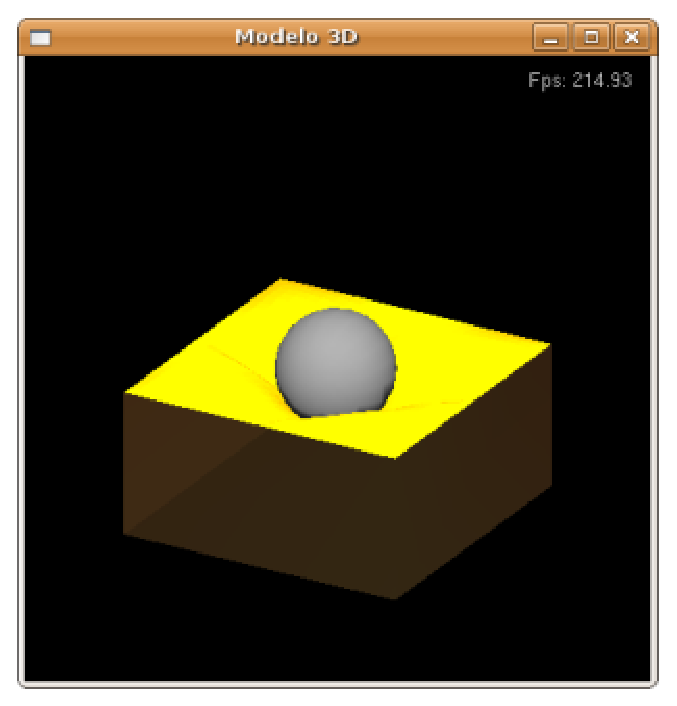
\includegraphics[width=0.85\textwidth]{Img/04/modeloPortada}
 \caption[Ejemplo del programa en ejecución]{Una imagen del programa que implementa el modelo.}
 \label{programa:portada}
\end{figure}

\subsubsection{Constantes del experimento}
En una situación como la antes descrita hay muchísimas variables del modelo, sin embargo al momento de hacer la implementación en código decidí dejar fijas algunas de ellas, es decir que la única manera de cambiarlas es modificando en el código fuente y recompilando el programa por completo.
Aquí está la lista de estas variables y su significado.

Las variables que se decidieron dejar fijas, y que por ende se convierten en constantes en el experimento son las siguientes:

\begin{itemize}
 \item El número de partículas por lado de la tela.
 \item Dimensiones (alto, ancho y largo) de la caja.
 \item La masa total de la tela. Y por lo tanto, la masa de cada partícula es ésta cantidad dividida entre el número total de partículas.
 \item El radio y la posición de la pelota.
 \item El tamaño del paso en el tiempo $\Delta t$ que se usa para los métods numéricos de integración.
\end{itemize}

Los valores de estas constantes con las que se hizo este experimento están en la tabla~\ref{valores:constantes}.
\begin{table}
\ra{1.2}
\begin{center}
\begin{tabular} {@{}lrp{10cm}@{}}
\toprule
Constante & Valor & Comentario\\ 
\midrule
 Número de partículas & 22 & Para que se vea mejor el modelo, se elige un número par\\
 Dimensiones caja & $0.75 \times 1.5 \times 1.5$ & Se forma una caja de tapas cuadradas \\
 Masa tela & 10 & La masa de cada particula es entonces $\frac{10}{22^{2}}$ \\
 Radio pelota & 0.25 &  \\
 Posición pelota & $(0, 1.5, 0)$& Como el cuerpo neumatico esta centrado en el origen. La pelota esta justo arriba de él en el centro\\
 $\Delta t$ & 0.0025 & Determinado experimentalmente \\
\bottomrule
\end{tabular}
\caption[Tabla con los valores de las constantes durante el experimento]{Valor de las constantes del experimento}
\label{valores:constantes}
\end{center}
\end{table}

\subsubsection{Variables físicas del experimento}
La variables físicas del experimento pueden ser modificadas en tiempo de ejecución por medio del menú que muestra en la Figura~\ref{programa:menu}.

\begin{figure}
 \centering
 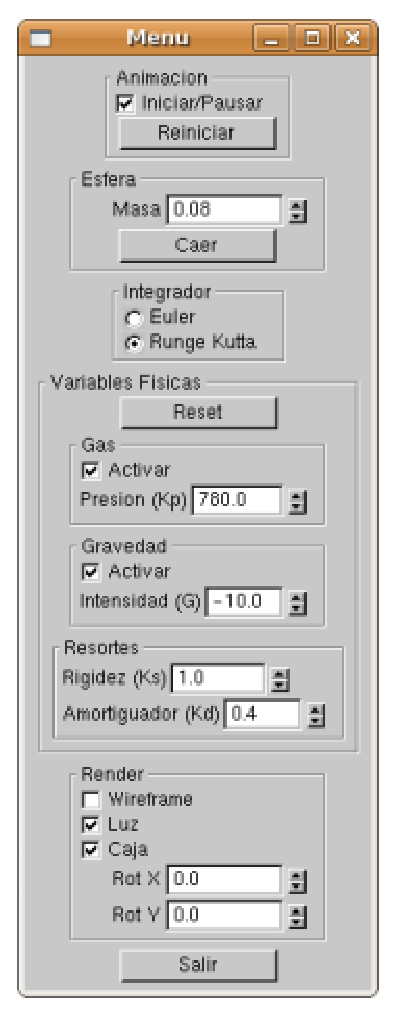
\includegraphics[width=0.5\textwidth]{Img/04/menu}
 \caption[Menú de usuario del programa]{Menú de usuario.}
 \label{programa:menu}
\end{figure}

Para la pelota o esfera (\emph{\textenglish{Sphere}}) que se refiere al cuerpo rígido.
la única variable que se puede modificar es su masa.

Los parámetros del cuerpo flexible que es posible modificar se dividen en tres subcategorias una por cada fuerza que se acumula.

La categoria del \emph{Gas}, al que se puede prender o apagar por medio del checkbox \emph{\textenglish{Pressure}}. 
Además, se puede modular su magnitud variando el valor de la constante $k_{g}$, por medio del control.

La de la \emph{\textenglish{Gravity}}, que al igual que la anterior se puede prender o apagar con el control  y también se puede modular variando el valor de la constante $g$.

Por últim subcategoria es la debida al resorte amortiguador (\emph{\textenglish{Spring-Damper}}.)
Esta fuerza no se puede apagar, pero se puede variar modificando dos parámetros $k_{s}$, que, como ya se dijo, controla la rigidez del resorte y $k_{d}$ que controla el amortiguamiento o pérdida de energía debida al resorte.

Aunque no es propiamnete una opción de la física. El menú tambien permite elegir que método numérico usar para integrar.
Las opciones disponibles son: \emph{Euler} y \emph{Runge-Kutta}.

Los valores de default de estas variables (el valor que tiene al iniciar la ejecución) son los que muestra la Tabla~\ref{valores:variables}.

\begin{table}
\ra{1.2}
\begin{center}
%\begin{tabular} {|c|c|p{10cm}|}
\begin{tabular} {@{}llp{10cm}@{}}
\toprule
Parametro & Valor & Comentario\\
\midrule
 Masa & 0.08 & Masa del cuerpo rígido \\
 Integrador & Euler & Método Numérico con el que se integra. \\
 Gas & Activado & El programa empieza con la fuerza del gas prendida \\
 $k_g$ & 17 & Constante de presión del gas \\
 Gravedad & Activada & La gravedad está activada \\
 $g$ & -10.0 & La gravedad es negativa (jala hacia abajo) \\
 $k_s$ & 100 & La fuerza de los resortes \\
 $k_d$ & 5 & El valor de damping \\
\bottomrule
\end{tabular}
\end{center}
\caption[Tabla con los valores de defecto de los parámetros]{Valor inicial de los parámetros del experimento}
\label{valores:variables}
\end{table}

\subsubsection{Opciones de control y visualización}
Hay otras opciones que se pueden modificar por medio del menú, que se refieren más a como controlamos la animación y a como se ve el modelo que a la física.

Dentro de las del flujo de la animación, sólo hay dos controles, el de \emph{\textenglish{Pause/Play}}, que puede detener (reanudar) la animación física (se sigue pudiendo mover la cámara).
Y el botón de \emph{\textenglish{Reset}}, que devuelve a todos los objetos a su posición original.

El botón de \emph{\textenglish{Drop}}, hace que la esfera se deje caer.

Dentro de la categoría de \emph{\textenglish{Render}}, se encuentran las siguientes opciones:

La primera opción \emph{\textenglish{solid}}, usa el modelo de iluminación de Phong (los materiales se obtiene de texturas) para dibujar todos los objetos en la escena.

Y la segunda opción \emph{\textenglish{wireframe}}. 
Que solo cambia la manera de dibujar el cuerpo neumático.
Dibuja con lineas azules las orillas de la caja y dibuja en una escala de color entre amarillo y rojo, los resortes (como lineas) y las particulas (como puntos) que forman el cuepor flexible.
El color asignado depende de la magnitud de la fuerza que actua sobre ellos.

Finalmente, además del menú de usuario, hay opciones que solo se pueden modificar por medio del \textenglish{mouse} y del teclado.

\begin{itemize}
 \item Arrastar el mouse con el botón izquierdo presionado, permite modificar el ángulo de la camara. Se usa el modelo de \emph{\textenglish{trackball camera}}.
 \item La rueda del mouse, cambia el \emph{\textenglish{zoom}} de la cámara.
 \item Presionar la tecla `\emph{s}' en el teclado toma un \emph{\textenglish{screenshot}}. Las imágenes son guardadas en el folder \mintinline{cpp}{Screenshoots} (Que debe ser creado por el usuario) en el mismo folder donde esta el ejecutable.
 \item Presionar \emph{Escape} en el teclado termina la ejecución del programa.
 \item Presionar la tecla `\emph{m}' muesta/oculta el menú de usuario.
 \item Presionar \emph{F11} cambia entre el modo de pantalla completa y de ventana.
 \item La tecla `\emph{p}' es un atajo para el boton de \emph{\textenglish{Play/Pause}} de la animación.
 \item La tecla `\emph{r}' es un atajo para el boton de \emph{\textenglish{Reset}} de la animación.
\end{itemize}

\subsection{Características del entorno de pruebas}

\subsubsection{Software}

El programa fue desarollado en lenguaje C++ y los shaders que sirven para hacer el render fueron escritos en GLSL.

Para poder compilar el código fuente de este programa es necesario tener un entorno de programación que contemple lo siguiente:

\begin{itemize}
 \item Un compilador de C++.
 \item La biblioteca OpenGL
 \item La biblioteca glfw
 \item La biblioteca Dear Imgui.
 \item La biblioteca GLM
 \item La biblioteca GLEW
 \item La biblioteca GLM
 \item La biblioteca FreeImage
 \item La biblioteca Assimp
\end{itemize}

Todas éstos requerimeintos son software libre (Mas detalles de esto en el Apéndice).
Aunque este trabajo fue desarollado en su totalidad en un sistema operativo GNU/Linux, todos los requerimeintos tienen la enorme ventaja de estar disponibles en cualquier plataforma.
Si las bibliotecas están correctamente instaladas, el programa y debe compilar y funcionar bajo cualquier sistema operativo.

\subsection{Hardware}
La mayoría de las pruebas fueron hechas en una laptop personal MSI GF65, con las siguientes características.

\begin{itemize}
\label{maquina:trabajo} 
 \item Procesador: Intel Core i7-9750H CPU @ 2.60GHz $\times$ 12.
 \item Memoria: 32GB DDR2.
 \item Tarjeta de Video: Nvidia GeForce GTX 1660 Ti Mobile\footnote{Aunque la laptop tiene la tarjeta de video descrita, el programa es tan simple que de hecho puede ejecutarse en la tarjeta de video integrada del procesador Intel sin problemas (Ver Figura~\ref{programa:menu})}.
 \item Sistema Operativo: Ubuntu 20.04 64bits.
\end{itemize}

Esto no quiere decir que este sea el hardware mínimo, sólo que la \emph{mayoría} de las pruebas se realiaron en este hardware.
Sin embargo, se ha ejecutado con éxito en equipos bastante accesibles. 
Éste trabajo es de hecho una reedición, el trabajo original se desarollo usando una laptop convencional en el año 2008.
Actualmente, éste programa debe poder ejecutarse en cualquier computadora personal, de escritorio o equipo movil sin problemas de capacidad del \emph{\textenglish{hardware}}.
Hoy en día la única limitante (de existir) podría acaso ser el \emph{\textenglish{software}}.

\section{Características físicas del modelo}
Para poner en a prueba la fidelidad del modelo, se hicieron las siguientes pruebas.
La mayoría para probar la sensibilidad del programa ante la variacion de sus parámetros físicos.

\subsection{Probando la gravedad}
La gravedad es la única fuerza que actúa tanto en el cuerpo flexible como en en el cuerpo rígido. Para entender mejor cómo afecta se sugieren las siguientes pruebas.

Partiendo de los valores de \emph{\foreignlanguage{english}{default}}, se espera a que la tela se estabilice (Figura~\ref{fig:testGEstable}).
Ahora se \emph{aumenta} la gravedad a su valor más \emph{pequeño} (recordemos que hacer la gravedad más fuerte es hacerla más negativa), es decir, $g=-20$, se observa ahora como la gravedad es muy fuerte como para que la presión del gas infle la tela, por lo que queda colgando un poco.
Las partículas que forman el cuerpo flexible son muy pesadas (son jaladas con más fuerza hacia abajo).
Esta situación se muestra en la Figura~\ref{fig:testGAumenta}. 
Ahora se deja caer la pelota y se espera que se estabilice de nuevo el programa, (Figura~\ref{fig:testGCae}) la gravedad hace que la pelota y las partículas pesen más, sin embargo la fuerza del gas que no se ha tocado compensa de alguna manera y no deja que se hunda más la pelota.
Con la pelota estable sobre la tela, apagué la fuerza del gas.
Al apagar la fuerza que equilibraba la gravedad todo se va hacia abajo, por la gravedad, pero como además esta fuerza es grande, la rigidez del resorte es poca para evitar un efecto de súper elongación como el que se ve en la Figura~\ref{fig:testGNoPres}, donde la pelota es detenida por el piso.

\begin{figure}
 \centering
  \begin{subfigure}[b]{0.45\textwidth}
    \includegraphics[width=\textwidth]{Img/04/gravity1}
    \caption{La tela se estabiliza con la gravedad y la presion.}
    \label{fig:testGEstable}
  \end{subfigure}
~
  \begin{subfigure}[b]{0.45\textwidth}
    \includegraphics[width=\textwidth]{Img/04/gravity2}
    \caption{La gravedad aumenta a $g=-20$}
    \label{fig:testGAumenta}
  \end{subfigure}
\\
  \begin{subfigure}[b]{0.45\textwidth}
    \includegraphics[width=\textwidth]{Img/04/gravity3}
    \caption{La pelota se deja caer.}
    \label{fig:testGCae}
  \end{subfigure}
~
  \begin{subfigure}[b]{0.45\textwidth}
    \includegraphics[width=\textwidth]{Img/04/gravity4}
    \caption{Se apaga la fuerza de presión}
    \label{fig:testGNoPres}
  \end{subfigure}
 \caption[Experimento: Fuerza de gravedad]{Probando la fuerza de gravedad} 
 \label{fig:testGravity}
\end{figure}

Reinicie la animación y vuelva a los valores de \emph{\foreignlanguage{english}{default}}.
De nuevo espere a que se estabilice la tela ahora disminuya la gravedad a su máximo valor posible, es decir una gravedad positiva: $g=1$.
Ahora verá que la tela se va más hacia arriba, como si se inflara más el cuerpo flexible, esto se debe a que ahora la gravedad no se opone a la presión del gas, sino mas bien le favorece, por lo que el cuerpo flexible, es jalado hacia arriba aún más, como se ve en la Figura~\ref{fig:testGpos1}.
Ahora deje caer la pelota, como la gravedad es positiva y pequeña (su valor absoluto en una décima parte del valor normal) la pelota \emph{sube lentamente}, y se aleja del cuerpo flexible (Figura~\ref{fig:testGpos2}).
La constante de gravedad influencía la velocidad de caída de los cuerpos.

\begin{figure}
 \centering
  \begin{subfigure}[b]{0.45\textwidth}
    \includegraphics[width=\textwidth]{Img/04/positiveGravity1}
    \caption{La presion y la gravedad jalan la tela hacia arriba.}
    \label{fig:testGpos1}
  \end{subfigure}
~
  \begin{subfigure}[b]{0.45\textwidth}
    \includegraphics[width=\textwidth]{Img/04/positiveGravity2}
    \caption{La pelota también es jalada hacia arriba}
    \label{fig:testGpos2}
  \end{subfigure}
 \caption[Experimento: $g > 0$]{La fuerza de gravedad cambia de signo} 
 \label{fig:positiveGravity}
\end{figure}

Por último vamos a reiniciar la animación y partiendo de los valores de \emph{\foreignlanguage{english}{default}} de los parámetros, se apaga la gravedad. 
Este comportamiento equivale a hacer $g=0$ con la diferencia de que se hacen menos cálculos, ahora vemos cómo de nuevo la tela se mueve hacia arriba, cómo la gravedad se oponía a la fuerza del gas y ya no está, el gas empuja la tela aún más hacia arriba.
Si en esta situación se deja caer la pelota no pasará nada, debido a que la caída de la pelota \emph{depende de la gravedad}, y al no haber, simplemente no hay caída.

Si primero se deja caer la pelota sobre la tela, y una vez que esta se estabiliza se apaga la gravedad, la pelota es empujada afuera del cuerpo flexible por un impulso. Ver la Figura~\ref{fig:noGravity}.

\begin{figure}
 \centering
  \begin{subfigure}[b]{0.3\textwidth}
    \includegraphics[width=\textwidth]{Img/04/gravityOff1}
  \end{subfigure}
~
  \begin{subfigure}[b]{0.3\textwidth}
    \includegraphics[width=\textwidth]{Img/04/gravityOff2}
  \end{subfigure}
~
  \begin{subfigure}[b]{0.3\textwidth}
    \includegraphics[width=\textwidth]{Img/04/gravityOff3}
  \end{subfigure}
 \caption[Experimento: Apagar la fuerza de gravedad]{La fuerza de gravedad es apagada después de que la pelota descansa sobre la tela.} 
 \label{fig:noGravity}
\end{figure}

\subsection{Probando la fuerza del gas}
Ahora se harán pruebas sobre la fuerza del gas. La fuerza del gas, por el diseño de nuestro experimento, se opone a la fuerza de gravedad, y actúa sólo sobre el cuerpo flexible, sin embargo tiene cierto efecto sobre la velocidad de las partículas del cuerpo flexible, que a su vez tienen cierto efecto sobre el cuerpo \emph{rígido} al momento de la colisión.

Inicie el programa con los valores de \emph{\foreignlanguage{english}{default}}, ahora apague la fuerza del gas y espere a que se estabilice el modelo, como se ve el la figura~\ref{pres:test1}.
Como no hay fuerza del gas, la tela o cuerpo flexible cuelga agarrada de las orillas de la caja.
Ahora deje caer la pelota sobre el cuerpo flexible y espere a que se estabilice la animación, justo como se ve en la figura~\ref{pres:test2}. 
Prenda la fuerza del gas y observe como la pelota es lanzada hacia arriba súbitamente como se ve en la figura~\ref{pres:test3}.

\begin{figure}
 \centering
 \includegraphics[]{Img/modPres1}
 \caption[Ejecución con la fuerza del gas apagada]{Fuerza del gas apagada.}
 \label{pres:test1}
\end{figure}

\begin{figure}
 \centering
 \includegraphics[]{Img/modPres2}
 \caption[Ejecución con la esfera cayendo en ausencia de fuerza del gas]{La pelota cae mientras está apagado el gas.}
 \label{pres:test2}
\end{figure}

\begin{figure}
 \centering
 \includegraphics[]{Img/modPres3}
 \caption[Ejecución con la esfera lanzada por la fuerza del gas]{La pelota es lanzada por la fuerza del gas.}
 \label{pres:test3}
\end{figure}

Otra prueba es ver los efectos de la variación de la constante $k_g$.
Inicie la animación con los valores de \emph{\foreignlanguage{english}{default}} y haga la constante $k_g$ pequeña, por ejemplo $k_g =$ 350.0; verá cómo el gas no es lo suficientemente fuerte para inflar el cuerpo flexible.
Ahora aumente poco a poco la constante $k_g$ y observe cómo se infla cada vez más el cuerpo flexible.
En la figura~\ref{pres:test4} se ilustran estas situaciones para diferentes valores en aumento de la constante $k_g$.

\begin{figure}
 \centering
 \includegraphics[]{Img/modPres4}
 \caption[Ejecución con diferentes valores de la constante de gas]{Variando la fuerza del gas: $k_g=$350.0 (arriba), $k_g=$730.0 (centro), $k_g=$970.0 (abajo)}
 \label{pres:test4}
\end{figure}

\subsection{Probando los resortes amortiguadores}
La siguientes pruebas sirven para mostrar cómo funcionan los resortes amortiguadores.
Primero vamos a hacer una prueba con la constante de \emph{\foreignlanguage{english}{damping}} $k_d$.
Como ya se dijo, el damping es una forma de perder energía del sistema y, por lo tanto, de eventualmente estabilizarse.
Iniciemos la animación con los valores de \emph{\foreignlanguage{english}{default}} y hagamos la constante $k_d=0$, es decir quitemos todo el \emph{\foreignlanguage{english}{damping}}.
Vemos que la tela empieza a oscilar rápidamente como consecuencia del gas.
Ahora quitemos también el gas y esperemos un momento; veremos como la tela oscila sin detenerse ni estabilizarse en ningún momento, es cierto que cada vez oscila menos, pero ciertamente tardará mucho en detenerse (o nunca se detendrá).

En la figura~\ref{res:test1}, podemos ver diferentes oscilaciones sin control por falta de un amortiguador.
Como ya se había dicho, el amortiguador agrega realismo (en la total ausencia de \emph{\foreignlanguage{english}{damping}}, el cuerpo flexible se ve poco real). La contra parte es que a mayor \emph{\foreignlanguage{english}{damping}}, también hay menos estabilidad numérica, por lo que el modelo es sumamente sensible al aumento en este parámetro.

Podemos ir aumentando el valor de $k_d$ poco a poco y ver cómo el modelo se vuelve inestable, podemos por ejemplo poner el máximo posible $k_d=$0.6 y reiniciar la animación, esperar a que se estabilice y apagar el gas, el modelo explota (ver figura~\ref{res:test4}).

Ahora analicemos la constante de rigidez $k_s$.
Esta constante hace a los resortes más poderosos, por lo que en general hace que las partículas que están unidas por ellos, se separen menos, es decir hace más estable el cuerpo flexible en general, además de prevenir el efecto de super elongación.

Iniciamos la animación con los valores de default y pongamos la constante del resorte $k_s$ a su máximo valor.
Ahora apaguemos el gas y vemos como la caída de la tela es menor, sin embargo al apagar y prender varias veces el gas también nos damos cuenta de que el cuerpo flexible parece oscilar más, como consecuencia de que los resortes en general jalan más fuerte, tanto hacia arriba como hacia abajo.

Ahora con la constante $k_s$ en el máximo y el gas prendido, vayamos poco a poco subiendo la presión del gas, aumentando $k_g$ hasta su máximo $k_g=$2000.0. 
Podemos ver cómo aun llegando al máximo de $k_g$, el cuerpo flexible se expande poco; esperemos a que se estabilice, como se ve en la figura~\ref{res:test5}. 
Ahora que tenemos el modelo estable y con ambas constantes $k_s$ y $k_g$ al máximo, poco a poco vayamos haciendo $k_s$ más pequeña y podremos apreciar como el cuerpo parece inflarse más (la resistencia de la membrana que lo mantiene unido es menor), como se ve en la figura~\ref{res:test6}, hasta llegar al momento donde explota ($k_s$ = 0.0).

\begin{figure}
 \centering
 \includegraphics[]{Img/modRes1}
 \caption[Ejecución sin fuerza de amortiguamiento]{Oscilación sin control: $k_d$=0.0}
 \label{res:test1}
\end{figure}

\begin{figure}
 \centering
 \includegraphics[]{Img/modRes4}
 \caption[Explosión por inestabilidad numérica]{La animación explota por inestabilidad numérica}
 \label{res:test4}
\end{figure}

\begin{figure}
 \centering
 \includegraphics[]{Img/modRes5}
 \caption[Ejecución con fuerza del gas y rigidez al máximo]{El gas está al máximo $k_g=$2000.0 al igual que la rigidez de los resortes $k_s=$2.0}
 \label{res:test5}
\end{figure}

\begin{figure}
 \centering
 \includegraphics[]{Img/modRes6}
 \caption[Ejecución con fuerza del gas y rigidez pequeña]{El cuerpo flexible se infla como consecuencia del gas la máximo y $k_s$ pequeña}
 \label{res:test6}
\end{figure}

\section{Presentación de resultados}

Una manera de medir la eficiencia tanto de la implementación como del modelo es ver cuánto se tarda en hacer los cálculos el programa antes de pintar un frame. 
Esta medida de rendimiento es calculada comúnmente en las simulaciones gráficas y por ello me decidí a implementarla.
Como ya se dijo, esto es dependiente del hardware, así que aquí presento dos tipos de análisis.

En la primera parte, se deja como constante el hardware, hago las pruebas en la misma computadora y se varían los cálculos que se hacen en la ejecución del programa.

En la segunda parte se mantienen constantes los cálculos en el programa y se ejecuta en varios ambientes de pruebas (diferentes máquinas y distintos sistemas operativos).

\subsection{Desempeño del programa}

La medida mas comúnmente usada es el número de cuadros que la aplicación pinta en un segundo o fps (de abreviar en inglés \emph{\foreignlanguage{english}{frames per second}}).
La rutina que calcula los fps se implementó con el siguiente código dentro de la función con el registro de callback idle.

\begin{verbatim}
frame++;
time = glutGet(GLUT_ELAPSED_TIME);
if (time - timebase > 1000) {
  fps = frame * 1000.0 / (time - timebase);
  timebase = time;
  frame = 0;
}\end{verbatim}

En donde la variable global \verb|frame|, ya fue inicializada la primera vez en ceros.
Esta rutina mide los frames por segundo, que después son desplegados en la parte superior izquierda de la pantalla.

Estas pruebas fueron realizadas en la máquina ya descrita antes en la sección~\ref{maquina:trabajo}.

Las variantes consideradas son las siguientes:

\begin{description}
 \item[Estado de la animación:]la animación puede estar en pausa o en movimiento, cuando está en pausa, se pueden cambiar la opciones de render y de la rotación de la cámara, pero el programa deja de hacer los cálculos del método numérico y por ende de la acumulación de fuerzas.
 \item[Hay colisiones:]la rutina de detección de colisiones siempre es ejecutada, sin embargo sólo en caso de que se detecte una colisión se llama a la rutina de respuesta de las colisiones.
 \item[Método Numérico:]el programa ejecuta uno de dos métodos numéricos para calcular el estado siguiente de la animación, puede ser por Euler o por Runge Kutta, de donde este último requiere de casi cuatro veces mas cálculos.
 \item[Fuerza del gas:]calcular la fuerza del gas requiere de hacer cálculos sobre el área y el volumen del cuerpo flexible, cuando esta fuerza está apagada, los cálculos se omiten.
 \item[Opciones de \emph{\foreignlanguage{english}{render}}:]las opciones del \emph{\foreignlanguage{english}{render}} hacen que se tengan que hacer cálculos de la iluminación y dar color a los objetos con base a dichos cálculos.
\end{description}

La nomenclatura de la prueba usando estas variables se especifica en el cuadro~\ref{nomenclatura:prueba}.

Cada una de las variantes arriba mencionadas puede tener dos valores.
El \emph{\foreignlanguage{english}{render}} puede tener muchos valores pero para hacer las pruebas sólo voy a considerar dos: prendido, cuando se dibujan todos los cuerpos en estado sólido con iluminación y apagado, cuando se dibuja en wireframe sin luz y no se dibuja la caja del cuerpo flexible.

\begin{table}
\ra{1.2}
\begin{center}
\begin{tabular} {@{}llp{10cm}@{}}
\toprule
 Variable & Valores & Explicación\\
\midrule 
 Animación & 0 ó 1 & Se considera 1 cuando la animación esta en marcha, y 0 cuando está en pausa. \\
 Colisiones & 0 ó 1 & Se considera 1 cuando hay una colisión y se ejecuta la respuesta, 0 cuando no hay colisión y sólo se ejecuta la detección. \\
 Método Numérico & 0 ó 1 & Se considera 1 cuando se ejecuta Runge Kutta y 0 cuando se ejecuta Euler. \\
 Fuerza del gas & 0 ó 1 & Se considera 1 cuando está prendida y 0 cuando está apagada. \\
 Render & 0 ó 1 & Se considera 1 cuando se hace la mayor cantidad render, como se explicó arriba y 0 cuando se hace el mínimo posible. \\
\bottomrule
\end{tabular}
\end{center}
\caption[Explicación de la nomenclatura de la prueba del programa]{Nomenclatura de la prueba}
\label{nomenclatura:prueba}
\end{table}

Se tienen pues cinco posibles variantes, cada una con dos valores.
Se ejecutaron los 18 casos posibles (la animacion apagada implica que haya opciones que no tengan sentido, por eso son sólo 18 en vez de 32) y para cada caso anoté entre qué valores oscilan los fps. Los resultados se resumen en la tabla~\ref{resultado:prueba1}.

La razon por la cual los fps, son un rango es que al momento de la ejecución, cada segundo varía el valor de los fps.
Es por eso que al hacer el experimento con las condiciones de cada caso, anote tanto el valor máximo que alcanzaron lo fps, como el valor mínimo; esto es lo que llamo el rango.

La columna de contribución, representa cuánto contribuye a los cálculos la prueba en cuestión con respecto a que se hacen \emph{todos} los cálculos, tomando como base el caso en que todas las variables están prendidas.
La contribución $C$ es calculada de la siguiente manera:

$$ C = \frac{FPS_{min} + FPS_{max}}{2} \div FPS_{base}$$

En donde $FPS_{min}$ es el mínimo de fps en cada categoría y $FPS_{max}$ es el máximo de fps en la misma, $FPS_{base}$ es el promedio de fps de la categoría base, para este caso $FPS_{base} =$ 210.81 dado que es el promedio de los $FPS$ de la prueba que más poder requiere y se presenta en el último renglón de la tabla.

\begin{table}
\ra{1.2}
\begin{center}
%\begin{tabular} {|c|c|c|c|c|c|c|}
\begin{tabular} {@{}cccccrr@{}}
\toprule
 Anim & Coli & Método & F. Gas & Render & FPS & Contr\\
\midrule
 0 & n/a & n/a & n/a & 0 & 2753.08 - 2768.15 & 0.08\\
 0 & n/a & n/a & n/a & 1 & 2754.01 - 2826.18 & 0.08\\
 1 & 0 & 0 & 0 & 0 & 654.35 - 663.34 & 0.32\\
 1 & 0 & 0 & 0 & 1 & 620.38 - 630.37 & 0.34\\
 1 & 0 & 0 & 1 & 0 & 501.04 - 512.98 & 0.42\\
 1 & 0 & 0 & 1 & 1 & 464.03 - 491.02 & 0.44\\
 1 & 0 & 1 & 0 & 0 & 447.99 - 456.54 & 0.47\\
 1 & 0 & 1 & 0 & 1 & 454.09 - 474.05 & 0.45\\
 1 & 0 & 1 & 1 & 0 & 240.52 - 251.99 & 0.86\\
 1 & 0 & 1 & 1 & 1 & 203.57 - 212.57 & 1.01\\
 1 & 1 & 0 & 0 & 0 & 640.72 - 660.54 & 0.32\\
 1 & 1 & 0 & 0 & 1 & 612.76 - 627.74 & 0.34\\
 1 & 1 & 0 & 1 & 0 & 499.03 - 512.03 & 0.42\\
 1 & 1 & 0 & 1 & 1 & 470.06 - 484.52 & 0.44\\
 1 & 1 & 1 & 0 & 0 & 347.31 - 357.29 & 0.60\\
 1 & 1 & 1 & 0 & 1 & 333.67 - 342.32 & 0.62\\
 1 & 1 & 1 & 1 & 0 & 214.34 - 219.26 & 0.97\\
 1 & 1 & 1 & 1 & 1 & 209.04 - 212.57 & 1.00\\
\bottomrule
\end{tabular}
\end{center}
\caption[Resultados de la prueba del programa]{Resultados primera prueba}
\label{resultado:prueba1}
\end{table}

Hay algunos datos interesantes con respecto a la tabla \ref{resultado:prueba1}, por ejemplo el hecho de lo poco que contribuye el render al desempeño de la animación (el .03).
Esto se explica por que cuando el render está apagado se trazan más objetos gráficos, se dibujan cuatro lineas y cuatro puntos por cada cara, mientras que cuando el render está prendido si bien se hacen cálculos de iluminación sólo se dibuja un cuadro por cada cara.

También de la tabla, puedo concluir  que lo que más contribuye al desempeño de la animación es el método numérico usado, pues como dijimos el
método de RK4, lleva casi cuatro veces más cálculos que el método de Euler (en la tabla se ve que representa el .56 de los cálculos).

El otro factor que hace considerablemente más lenta la animación es el cálculo de la fuerza del gas con el .48 del tiempo.

\subsection{Desempeño del programa en diferentes ambientes}

La última prueba consistió en hacer constante la ejecución del programa y ver qué desempeño tiene en diferentes tipos de hardware.

Para esta  prueba se ejecutó el programa en diferentes ambientes.
En cada ambiente se consideran importantes sólo las siguientes características: la memoria principal, el sistema operativo, el procesador, la arquitectura y si hay o no memoria de vídeo.

La ejecución del programa se hizo de una manera típica, lo que haciendo una equivalencia con la prueba anterior es que esté en marcha la animación, que haya colisiones con el método de Runge Kutta, que haya fuerza del gas y que el \emph{\foreignlanguage{english}{render}} se haga completo.
También se hizo la ejecución con las siguientes características mínimas: método de Euler y sin fuerza de gas.
De ambas pruebas se miden los fps.

Los resultados se listan a continuación.
\begin{itemize}
 \item Sistema Operativo: Ubuntu 7.04
 \item Procesador: Opteron 1214 a 2.2GHz
 \item Memoria RAM: 2.0GB
 \item Memoria de Video: Tarjeta Nvidia FX3500, 256MB, driver propietario
 \item Velocidad en prueba mínima: 612.76 - 627.74fps
 \item Velocidad en prueba normal: 209.04 - 212.57fps
\end{itemize}

\begin{itemize}
 \item Sistema Operativo: Windows XP professional edition
 \item Procesador: AMD Duron a 1.2GHz
 \item Memoria RAM: 512MB
 \item Memoria de Video: Tarjeta Nvidia 64MB
 \item Velocidad en prueba mínima: 72.0 - 102.0fps
 \item Velocidad en prueba normal: 60.0 - 94.0fps
\end{itemize}

La última prueba se llevó a cabo en una máquina virtual, con el fin de evaluar los requerimientos mínimos.

\begin{itemize}
 \item Sistema Operativo: Windows XP professional edition
 \item Procesador: Dual Core AMD Opteron 999Mhz
 \item Memoria RAM: 256MB
 \item Memoria de Video: Ninguna, adaptador VM-Ware SVG 2
 \item Velocidad en prueba mínima: 65.40 - 71.72fps
 \item Velocidad en prueba normal: 46.44 - 52.22 fps
\end{itemize}



\chapter*{Conclusiones}
\addcontentsline{toc}{chapter}{\numberline{}Conclusiones}
\markboth{CONCLUSIONES}{CONCLUSIONES}

Después de haber hecho pruebas y evaluado los resultados obtenidos presento las siguientes conclusiones.

Lo más importante es que las ecuaciones diferenciales, permiten modelar gráficamente el comportamiento físico de un cuerpo neumático que interactúa con un cuerpo rigido, en tiempo real.
También hay que recalcar que este modelo es tiene sustento en la física, es decir es un modelo basado en física y no en geometría.

Creo también que la técnica aquí usada, la de utilizar un gas ideal dentro del cuerpo flexible, es muy buena para enfrentar este tipo de problemas pues nos da todo lo que desearíamos de una animación: es computacionalmente barata, al menos lo suficiente para alcanzar tiempo real y es físicamente adecuada para modelar el gas.

El modelo como se describe depende poco del poder gráfico, es decir el render sigue siendo una operación relativamente barata \emph{en comparación} con los cálculos numéricos.
Dentro de los cálculos numéricos, lo que más contribuye es el método numérico de Runge Kutta seguido de la acumulación de la fuerza del gas.

Si bien el utilizar el método de Euler, hace considerablemente más rápido de ejecutarse el programa, recomiendo usar el método de Runge Kutta, por mayor estabilidad ante la variación de las constantes, lo que se traduce en la posibilidad de mayor interacción.
También creo que este método no es tan complejo de implementar.

El \emph{\foreignlanguage{english}{damping}} es un parámetro que debe de estar presente, sin embargo requiere tener mucho cuidado al determinar un valor adecuado, considero que el valor más adecuado es el más grande posible sin que la animación explote.
Este modelo es muy sensible a las variaciones aun \emph{pequeñas} de este parámetro.

Se recomienda ampliamente que al momento de programar se tome tiempo para hacer una adecuada elección de las estructuras de datos.
Guardar todo en una estructura de datos lineal, simplifica bastante la programación. De igual manera, recomiendo tener diferentes maneras de acceder a las propiedades de las partículas, ya sea por los resortes o por medio de las caras.

El modelo del gas ideal es un modelo muy recomendado para simular cuerpo flexibles; con una adecuada elección de los parámetros se puede tener un comportamiento bastante realista.
Por lo que considero que el objetivo fundamental de este trabajo se cumple.

Hay muchas mejoras posibles para esta implementación, pienso que hay campo para futuras investigaciones en los siguientes detalles:

\begin{itemize}
 \item El cálculo del volumen del cuerpo flexible.
 \item Investigar sobre un método numérico más eficiente, aquel que dé más rapidez sin perder estabilidad.
 \item El manejo de colisiones más eficiente.
\end{itemize}

Para hacer el cálculo del volumen en~\cite{Matika:SoftBody} se propone hacer uso del \emph{teorema de divergencia}.
Considero que este podría ser un buen camino para hacer más flexible el cálculo del volumen y del área.

Para el método numérico se hicieron pruebas con el integrador de Verlet, sin embargo abandoné ese camino porque en un esquema como éste no se toma en cuenta la velocidad de la partícula, por lo que no encontré manera de responder a las colisiones.
Creo que investigar la manera de incluir una fuerza de impulso como respuesta a la colisión y utilizar el integrador de Verlet daría resultado.

Hay también que considerar una respuesta a las colisiones que conlleve una pérdida de energía al momento de la colisión.
Es decir, eliminar el supuesto de colisiones perfectamente elásticas.
Aunque escribí en el segundo capítulo sobre ellas, no fueron implementadas en el programa.

Mi forma de manejar tanto la detección como la respuesta de las colisiones  no es la más eficiente, pues pruebo una a una las partículas del cuerpo flexible.
Algún algoritmo que probara sólo las partículas cercanas haría mejor la detección.

También hay una mejora posible si se considera que el cuerpo flexible puede colisionarse consigo mismo, es decir probar colisiones de las caras del cuerpo con cada una de las partículas y luego responder la colisión.
Considero que en cualquier configuración del cuerpo flexible que no sea un volumen convexo este problema estará presente.



\begin{appendix}
\appendix
\chapter*{Apéndice: Sobre el software libre}
\addcontentsline{toc}{chapter}{Apéndice}
\markboth{APENDICE}{APENDICE}
Un objetivo secundario cuando empecé a hacer esta tesis, fue que toda ella fuera hecha con Software Libre. Al final tengo que admitir que esto no fue llevado a cabo por completo, pues todas las figuras del primer capítulo con la excepción de la~\ref{OsciAmor:fig} fueron hechas en AutoCAD (http://www.autodesk.es).

Aun así, pienso que este objetivo se cumplió parcialmente, pues fuera de lo antes mencionado todo se hizo en Software Libre; el desarrollo del programa fue hecha sobre GNU/Linux en particular sobre la distribución Ubuntu (www.ubuntu.com).

Para programar se utilizó gcc (http://gcc.gnu.org/), junto con Mesa (http://www.mesa3d.org/) y freeglut (http://freeglut.sourceforge.net/), la biblioteca glui (http://www.cs.unc.edu/rademach/glui/) también es software libre. Como IDE utilice Geany (http://geany.uvena.de/) y debo decir que estoy muy satisfecho con él.

Cuando hubo necesidad de hacer pruebas en Windows, también se ocuparon programas libres: se compiló con Dev-C++ (http://www.bloodshed.net/devcpp.html) como IDE y con Migwn (http://www.mingw.org/) como compilador junto con glui y freeglut.

El texto de la tesis se escribió en \LaTeX, en Ubuntu utilice tetex (http://web.bilkent.edu.tr/History/valley/tetex-index.html)y en Windows miktex (http://miktex.org/).

También fue de muchísima ayuda contar con un repositorio para guardar los avances del proyecto, esto me dio la enorme ventaja de poder trabajar en cualquier computadora que tuviera acceso a internet. Para eso se hizo uso de apache (http://www.apache.org/) y de subversion (http://subversion.tigris.org/).

\end{appendix}



\addcontentsline{toc}{chapter}{Bibliografía}

\bibliographystyle{plain}
\thispagestyle{empty}

\bibliography{bibliografia}
\nocite{*}

\end{document}
